\documentclass[12pt,a4paper]{report}
\usepackage[a4paper,margin=1in]{geometry}
\usepackage[hidelinks]{hyperref}
\usepackage{caption}
\usepackage{graphicx}
\usepackage{lmodern}
\usepackage{setspace}
\usepackage{titlesec}
\usepackage{lipsum}
\usepackage{fancyhdr}
\usepackage{xcolor}
\usepackage{float}
\usepackage{tcolorbox}
\usepackage{amssymb}
\usepackage{amsmath}
\usepackage{algorithm}
\usepackage{algorithmic}
\usepackage{pifont}
\usepackage[Sonny]{fncychap}

\captionsetup{font=small} 

\newcommand{\todo}[1]{%
  \par\noindent%
  \begin{tcolorbox}[colback=yellow, colframe=black, boxrule=0.5pt, sharp corners, width=\linewidth, before skip=5pt, after skip=5pt]
    \textbf{TODO:} #1
  \end{tcolorbox}%
  \par
}

\newcommand{\answer}[1]{%
  \par\noindent%
  \begin{tcolorbox}[colback=blue!10!white, colframe=blue!80!black, boxrule=0.5pt, sharp corners, width=\linewidth]
    \textbf{ANSWER:}~#1
  \end{tcolorbox}%
}

% REMARK (orange with ! icon)
\newcommand{\remark}[1]{%
  \par\noindent%
  \begin{tcolorbox}[ colback=orange!20!white, colframe=orange!80!black, boxrule=0.5pt, sharp corners, width=\linewidth, ]
    {\textbf{\textcolor{orange!80!black}!REMARK:}}~#1
  \end{tcolorbox}%
}

%--------------------------------
% Chapter Title
%--------------------------------
\ChNameVar{\raggedleft\bfseries\Large}   % "CHAPTER" word
\ChNumVar{\raggedleft\bfseries\Large}    % Chapter number
\ChTitleVar{\raggedleft\bfseries\Large}  % Chapter title

%--------------------------------
% Section Title
%--------------------------------
\titleformat{\section}[block]
    {\titlerule[2pt]\addvspace{0.8ex}%
    \bfseries\Large}
    {\thesection}{0.5em}
    {}[{\addvspace{0.4ex}\titlerule[2pt]}]
\titlespacing{\section}{0pt}{*4}{*4}

% Display current section in header:
\pagestyle{fancy}
\fancyhf{}
\fancyhead[L]{\nouppercase{\rightmark}}
\fancyfoot[C]{\thepage}

\begin{document}

% Title Page
\begin{titlepage}
    \centering
    
    % University logo at the top
    
\includegraphics[width=0.3\textwidth]{images/uantwerpen_logo.jpg}\\[1cm]
    
    {\Huge \textbf{Multimodal Data Integration for Predictive Modelling of Measles Vaccine Response with Cross-Vaccine Marker Validation}} \\
    \vfill
    
    {\Large \textbf{Elias Dams}}\\[1cm]
    
    \textbf{Promotor:} Dr. Pieter Meysman\\
    \textbf{Supervisor:} Fabio Affaticati\\[1.5cm]
    
    {\Large \textbf{University of Antwerp}}\\
    {\large Faculty of Science}\\[0.5cm]
    
    \textbf{2024-2025}\\[1.5cm]
    
    Submitted in fulfilment of the requirements for the degree of\\
    \textbf{Master in Computer Science: AI \& Data Science}\\[1cm]
    
    \textbf{June 2025}\\[2cm]
    
    % Decorative line at the bottom
    \vfill
    
\includegraphics[width=1.0\textwidth]{images/bottom_design.jpg}

\end{titlepage}

% remove page numbering
\pagenumbering{gobble}

% Table of Contents
\tableofcontents
\newpage

% List of Figures, Tables, Acronyms
\listoffigures

\listoftables

\chapter*{List of Acronyms}
- TCR: T-cell receptor

% Preliminary Sections
\chapter*{Summary}

\chapter*{Acknowledgements}

\chapter*{Abstract}




\chapter{Introduction}
% put page numbering back on
\pagenumbering{arabic}
\setcounter{page}{1}
%%%%%%%%%%%%%%%%%%%%%%%%%%%%%%%%%%%%%%%%%%%%%%%%%%%%%%%%%%%%%%%%%%%%%%%%%%%%%%%%%%%%%%%%%%%%%%%%%%%%%%%%%%%%%%%%%%%%%%%%%%%%%%%%%%%%%%%%%%%%%%%%%
% \todo{Introduce the research problem, significance of predictive modeling for vaccine response, and an overview of the multimodal data integration approach.}
% \remark{Maybe a citation here https://pmc.ncbi.nlm.nih.gov/articles/PMC5861809/} - Fabio

Vaccination is widely recognized as one of the most cost‑effective public health strategies, yet individuals exhibit significant variability in their immune responses. Foundational studies in systems immunology \cite{castrucci2018factors,brodin2017human} have shown that while vaccines like yellow fever and influenza generally trigger robust immune responses, the intensity of these responses (such as antibody production) can vary considerably. This variability is especially noticeable among very young or very old individuals, or those with other health issues, because their immune systems tend to be less robust and more unpredictable.\\
\\
%This thesis takes a data‑driven, computer science approach to predict responses to the measles (\remark{I would call it the MMR (Measles Mumps and Rubella trivalent vaccine, like you call it afterwards}Rubeola) 
This thesis takes a data‑driven, computer science approach to predict responses to the MMR (Measles, Mumps, and Rubella) trivalent vaccine using multimodal data integration, meaning that it combines different types of data (each representing a distinct aspect of the immune response) into a single, unified analysis. Measles is a highly contagious viral disease characterized by fever and a red rash, and it can lead to serious complications like pneumonia, particularly in infants and young children \cite{moss2017measles}. In this thesis, the immune response is primarily evaluated based on antibody titers, which are regarded as the gold standard for assessing vaccine effectiveness because they offer a precise, quantifiable measure of the immune system’s capacity to generate protective antibodies \cite{plotkin2010correlates} (see Section~\ref{sec:antibody_titers} for further details). The goal is to develop predictive models that not only forecast individual vaccine responses but also identify specific immune markers that consistently correlate with vaccine effectiveness across various vaccines. A process known as cross‑vaccine marker validation.\\
\\
Predictive modeling is essential because it allows anticipation of an individual’s vaccine response well before the full immune reaction is measured. For example, Van Tilbeurgh et al. (2021) \cite{vanTilbeurgh2021predictive} demonstrated that combining high‑throughput technologies (such as transcriptomics, proteomics, and \textit{in vivo} imaging) with computational models can reveal immune signatures linked to vaccine efficacy. Such models support personalized vaccination strategies by allowing healthcare providers to tailor vaccine schedules, dosages, or even select alternative vaccines based on predicted responses. For instance, if a model indicates a low immune response based on specific genetic markers, healthcare providers might opt for an additional booster or an adjusted formulation. Ultimately, this targeted strategy not only optimizes vaccine efficacy but also ensures better resource allocation.\\
\\
% \todo{@Fabio info about the study my data is coming from.}
% \remark{doi of the original study 10.1016/j.vaccine.2020.03.004} - Fabio

%The initial measles dataset used is derived from the study \remark{simply citing the first author and the date is fine} “Transcriptomic profiling of different responder types in adults after a Priorix$^{\mbox{\scriptsize\textregistered}}$ vaccination” \cite{bartholomeus2020transcriptomic}. 
\noindent
The initial measles dataset used is derived from the study by Bartholomeus et al. (2020) \cite{bartholomeus2020transcriptomic}.
In this study, adult volunteers (23 females and 17 males, aged between 19 and 29 years, all of whom were previously primed with MMR vaccines in childhood) received a booster dose of Priorix$^{\mbox{\scriptsize\textregistered}}$ and were monitored at four time points (Day 0, Day 21, Day 150, and Day 365) to measure antibody titers and gene expression profiles. In this thesis, the focus will be concentrated specifically on the measles-related data from this dataset. \\
%For a detailed exploration of the dataset’s biological composition and characteristics, refer to Section~\ref{sec:biological_characterization_of_the_dataset}.\\
\\
Nevertheless, several challenges must be addressed to realize the full potential of predictive modeling. One challenge in this research is that the dataset comprises only 40 samples. This small sample size limits statistical power and increases the risk of overfitting, making it difficult to generalize the model to a broader population. In addition, the project involves integrating heterogeneous data types, such as cytokine levels, cytometry data, T cell receptor sequences, and RNA profiles. These different modalities come with varying scales and units, which adds complexity to data normalization and feature selection. Moreover, any noise or missing values in a small dataset can have a large impact on the model’s performance, potentially leading to biased results. The high number of features (in the RNA data) relative to the number of samples may require careful feature selection or dimensionality reduction to prevent the models from becoming too complex and overfitted. Finally, an additional challenge arises from the risk of data leakage during the feature selection process. Selecting features based on their relevance to the Hepatitis B response prior to model evaluation can introduce bias, artificially inflating performance metrics and ofcourse reducing generalizability.
%%%%%%%%%%%%%%%%%%%%%%%%%%%%%%%%%%%%%%%%%%%%%%%%%%%%%%%%%%%%%%%%%%%%%%%%%%%%%%%%%%%%%%%%%%%%%%%%%%%%%%%%%%%%%%%%%%%%%%%%%%%%%%%%%%%%%%%%%%%%%%%%%





\chapter{Background}
%%%%%%%%%%%%%%%%%%%%%%%%%%%%%%%%%%%%%%%%%%%%%%%%%%%%%%%%%%%%%%%%%%%%%%%%%%%%%%%%%%%%%%%%%%%%%%%%%%%%%%%%%%%%%%%%%%%%%%%%%%%%%%%%%%%%%%%%%%%%%%%%%
\todo{Cover key concepts in immunology and data science, review existing work on vaccine response modeling.}
\noindent
To understand the work presented in this thesis, it is essential to have a basic grasp of concepts from both immunology and data science. As a computer scientist, my approach is mainly data-driven, focusing on extracting, integrating, and analyzing various types of biological data. However, a foundational understanding of the underlying biological processes is critical to meaningfully interpret the results and validate the predictive models developed in this research.

\section{Background in Biology}

\subsection{Immune System Overview}

\begin{figure}[h]
  \centering
  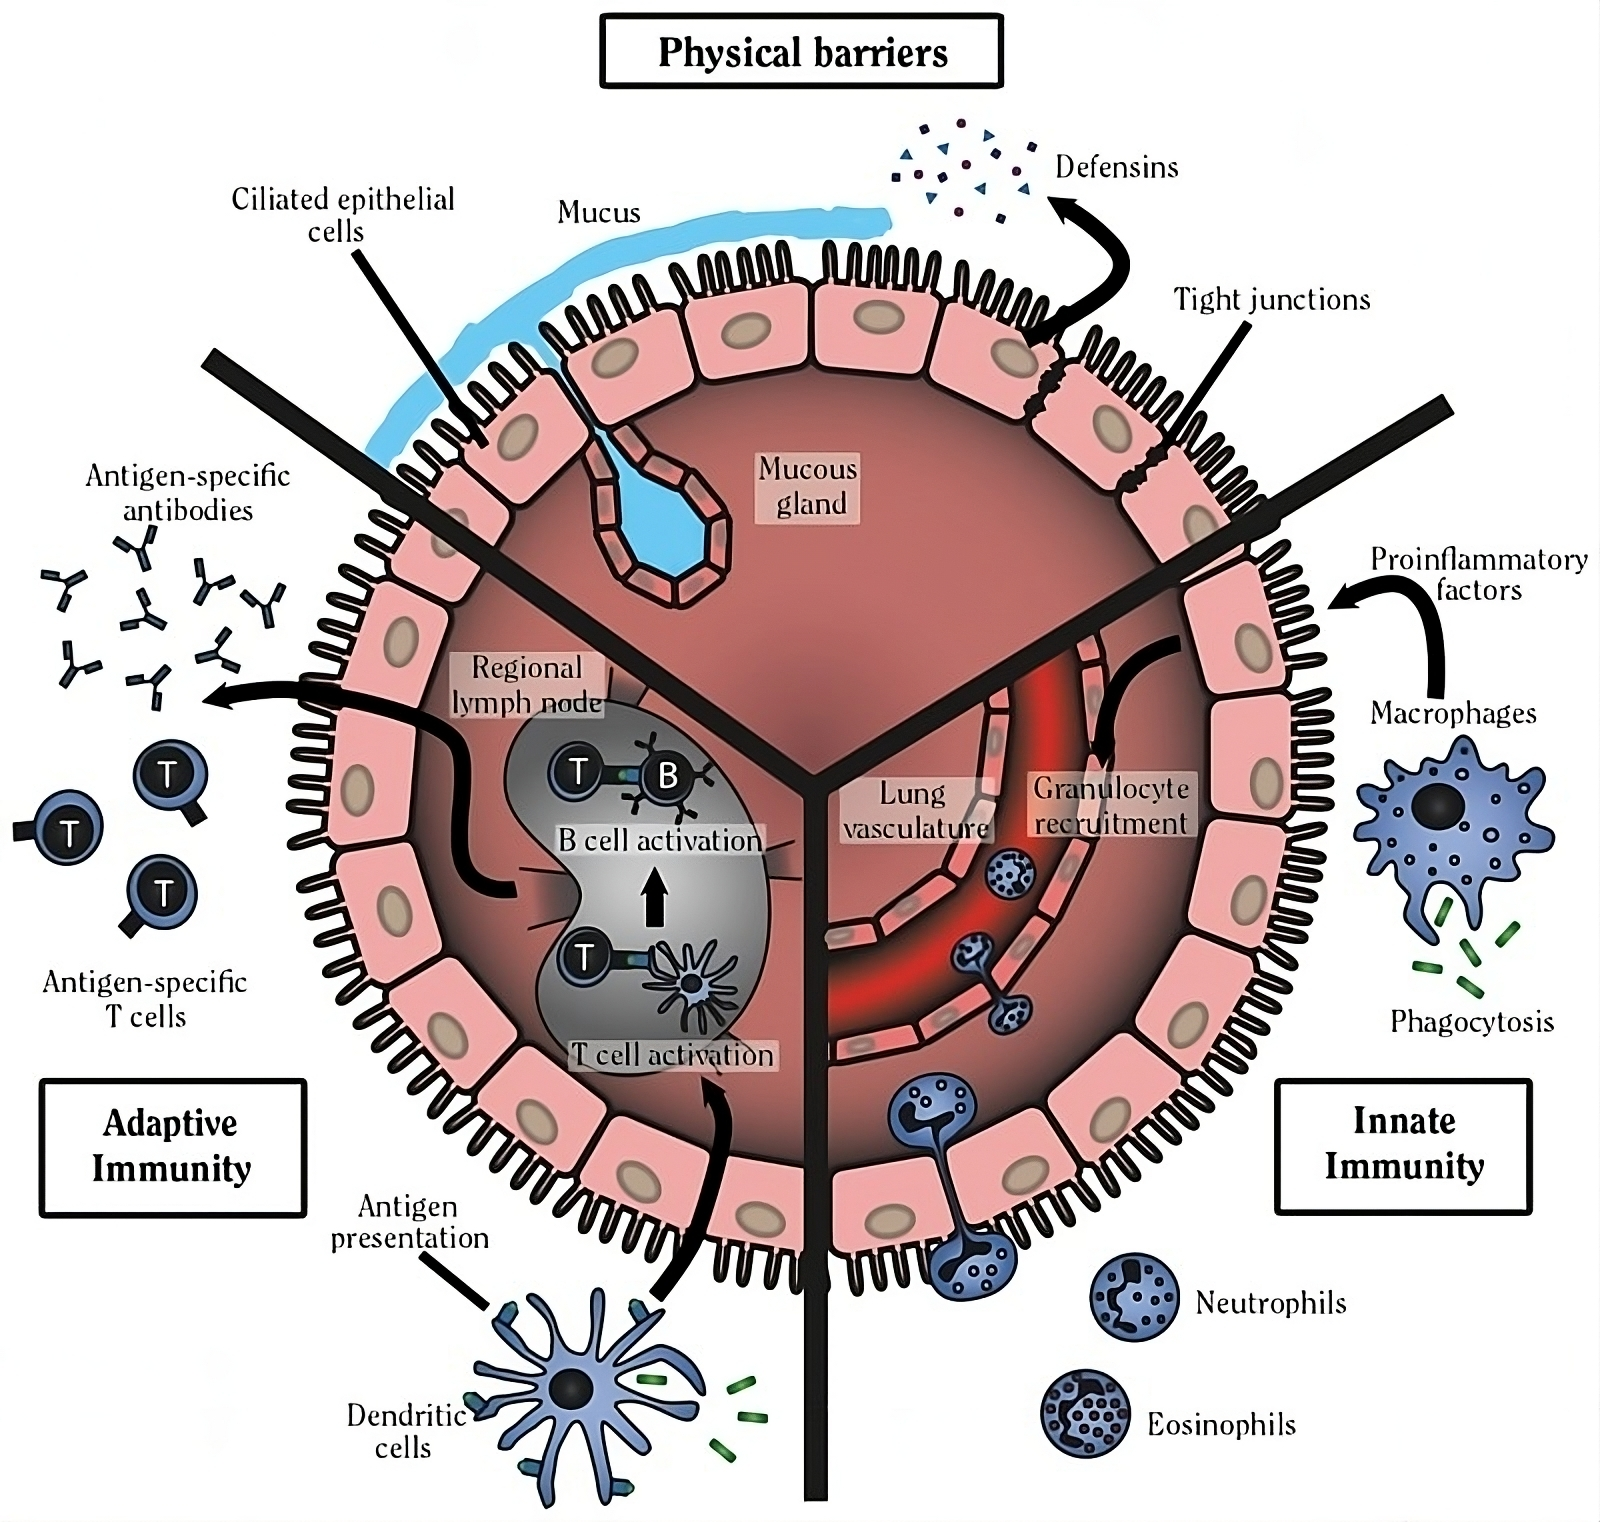
\includegraphics[width=0.9\textwidth]{images/Diagram_of_innate_and_adaptive_immunity.jpeg}
  \caption[Diagram of Innate and Adaptive Immunity]{Diagram showing physical barriers, innate immune cells (e.g., macrophages, dendritic cells, natural killer cells) and adaptive immune components (B and T cells) working together. Reproduced from Figure 10.5 in \emph{The Health Consequences of Smoking—50 Years of Progress: A Report of the Surgeon General} (2014) \cite{smoking2014}.}
  \label{fig:immunity}
\end{figure}
A key element of these biological processes is the functioning of the immune system, which can be broadly divided into three main components, as depicted in Figure \ref{fig:immunity}:\\
\\
\textbf{Physical barriers (top)}\\
Physical barriers, including the skin and mucous membranes, serve as the body’s first line of defense by blocking most pathogens (microorganisms such as viruses, bacteria, fungi, and parasites that can cause disease) from entering.\\
\\
\textbf{Innate Immunity (right)}\\
In case a pathogen still crosses the barriers, innate immunity comes into action. This defense is rapid and non-specific. Think of macrophages and neutrophils as cells that engulf invaders through a process called phagocytosis. Eosinophils and other granulocytes also attack pathogens or initiate inflammatory responses. Natural killer cells (NK cells) are also part of innate immunity and can directly destroy infected or abnormal cells. Although this response is very rapid, it does not recognize pathogens in the same specific way as the next branch. \cite{janeway2001immunobiology}\\
\\
\textbf{Adaptive Immunity (left)}\\
Acquired or adaptive immunity is the “slower but more targeted” defense. B cells play a crucial role by producing antibodies, which are proteins that bind to specific non-self antigens. These antibodies neutralize pathogens and tag them for destruction by immune cells such as phagocytes.
The concentration of these antibodies in the blood is measured as “antibody titers,” as mentioned earlier. Higher titers generally indicate a stronger immune response. T cells are also crucial and have several roles. They help coordinate the immune response (often referred to as “helper T cells”) and can directly kill infected cells (cytotoxic T cells). T cell receptors (TCRs), located on the surface of T cells and responsible for recognizing peptides presented by MHC I/II molecules, can be sequenced (see Figure\ref{fig:TCR_profiling}) to determine which T cell clones are activated in response to a vaccine. A major advantage of adaptive immunity is that it “learns” from previous exposure, allowing for much faster and more powerful immune responses in the event of repeated infection. This ability to form memory also underlies how vaccines work. \cite{janeway2001immunobiology}

\begin{figure}[h]
  \centering
  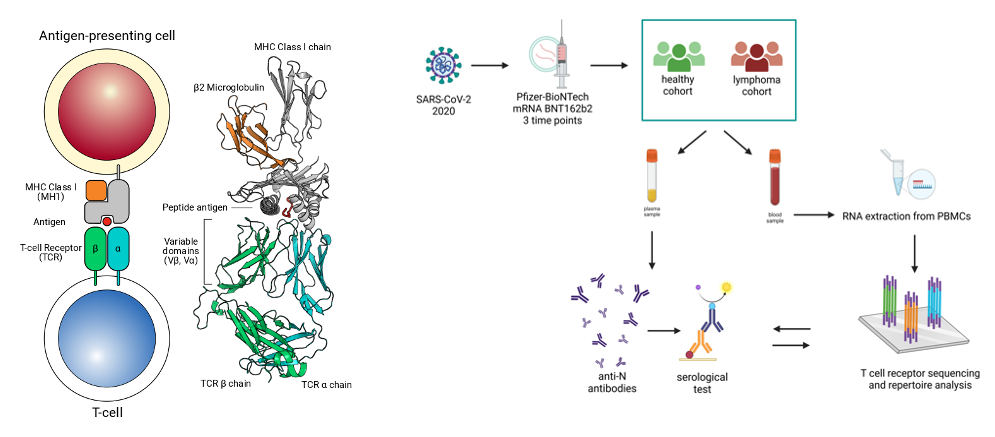
\includegraphics[width=1\textwidth]{images/TCR_profiling.png}
  \caption[ TCR sequencing Workflow]{Schematic outline of how TCR data is obtained from peripheral blood mononuclear cells (PBMCs) after vaccination. By extracting and profiling TCR sequences, it becomes possible to identify which T cell clones expand in response to the vaccine. This information provides insights into the breadth (diversity) and Depth (magnitude or intensity) of the adaptive immune response.}
  \label{fig:TCR_profiling}
\end{figure}

\noindent
Together, these three pillars provide a robust defence system that is able to successfully fight off most infections. It is also this dynamic between innate and adaptive immunity that determines the degree of vaccine response. The innate branch prepares the way, while the adaptive branch provides targeted antibodies and memory cells. This context is important because the predictive models developed here integrate features from both the innate and adaptive immune systems. For example, innate markers such as cytokine levels and certain cell counts can provide early signals about the body's general readiness to respond. Meanwhile, adaptive markers, such as TCR sequences of T cells, directly reflect the specific immune response that leads to antibody production after vaccination. Combining this data gives us a more complete picture of the immune landscape, allowing for better predictions of how effectively an individual will respond to the measles vaccine.

\subsection{Antibody Titers}
\label{sec:antibody_titers}
As mentioned above, antibody titers provide a quantitative measure of the concentration of specific antibodies in the blood, making them a reliable indicator of the immune system’s functional response against a pathogen \cite{plotkin2010correlates}. In essence, they reflect the “signal strength” of the response, with high titers indicating robust protection and low titers suggesting a weaker response. In this thesis, antibody titers serve as a crucial biomarker for classifying vaccine responses into strong and weak responders. 

\pagebreak
\section{Background in Computer science}
\todo{info about the used computer science techniques.}
\pagebreak
%%%%%%%%%%%%%%%%%%%%%%%%%%%%%%%%%%%%%%%%%%%%%%%%%%%%%%%%%%%%%%%%%%%%%%%%%%%%%%%%%%%%%%%%%%%%%%%%%%%%%%%%%%%%%%%%%%%%%%%%%%%%%%%%%%%%%%%%%%%%%%%%%





\chapter{Data Description and Preprocessing}
%%%%%%%%%%%%%%%%%%%%%%%%%%%%%%%%%%%%%%%%%%%%%%%%%%%%%%%%%%%%%%%%%%%%%%%%%%%%%%%%%%%%%%%%%%%%%%%%%%%%%%%%%%%%%%%%%%%%%%%%%%%%%%%%%%%%%%%%%%%%%%%%%
\todo{Detail the measles dataset (Cytokines, Cytometry, Clonal Breadth/Depth, RNA data) along with preprocessing steps taken.
Maybe i'll include a brief section here on hepatitis B preprocessing to set up the validation later.}
\noindent
In this chapter, I provide an overview of the measles dataset used in this study and outline the preprocessing steps required to prepare the data for analysis. The dataset integrates multiple biological modalities (including cytokine profiles, cytometry measurements, clonal breadth and depth of T cell receptors, and RNA sequencing data) to capture various aspects of the immune response to the measles vaccine. Additionally, I explain how response labels were assigned based on antibody titer trajectories, which serve as a key indicator of vaccine effectiveness. 

\section{Label Assignment Strategy}
% \todo{@Fabio How where they initially defined to be sure? And also where it general antibody titers or specific to measles, because it it is specific a friend who studies biomedical science said that high titers over the whole trajectory should be considered "responder".  }
% \remark{They are specific to Measles (we also have the ABs for the other 2 components as well). The problem is that these individuals were already primed/they already had received a stimulation to the antigens before thus some had preexisting antibody titers but they didn't grow after vaccination thus technically not having a response to the stimulus. From the original paper: "For classification of the immune responses, a hierarchical clustering method was applied on the antibody (Ab) titers at day 0 (prevaccination baseline) and days 21, 150 and 365 (post-vaccination). This clustering technique groups individuals with similar patterns in Ab titer evolution. This avoids using cut-off values, which may be biased. As shown in Figure 2, four different response groups were identified for each antibody titer: 159 (a) High Ab: individuals with a relatively high Ab titer before vaccination that remained stable or further 160 increased after vaccination (b) Low Ab: individuals with a relatively low Ab titer before vaccination that remained low after vaccination (c) Long response: individuals with a relatively low Ab titer before vaccination that increased after vaccination and stayed stable within the first year (d) Peak response: individuals with a relatively low Ab titer before vaccination that increased at day 21, and then decreased by day 150 and 365."}

\noindent
The original dataset included antibody titer measurements at four time points (Day0, Day21, Day150, and Day365), along with detailed qualitative classifications for each subject. These classifications, as noted in the original study \cite{bartholomeus2020transcriptomic}, were derived using a hierarchical clustering method that groups individuals based on similar patterns in antibody titer evolution, effectively avoiding potentially biased cut-off values. Specifically, the study identified four response groups: High Ab, Low Ab, Long response, and Peak response.\\
\\
It is important to acknowledge that these classifications, and the responder definition used in this study, are specific to measles. A significant factor in this dataset is the presence of pre-existing antibody titers due to prior exposure or vaccination. Consequently, some individuals with high pre-existing titers did not show an increase after vaccination, thus they don't technically respond to the stimulus.\\
\\
For the initial stages of modeling, I simplified the labels to a binary classification (\texttt{responder} and \texttt{non-responder}). Responders were defined as those whose antibody titers increased by at least 120 mIU/mL from Day0 to Day21, reflecting a widely accepted threshold for protective immunity against measles \cite{chen1990measles}. This simplification was done to create a more straightforward prediction task. However, the complexity of the original four classifications will be considered for future modeling refinements.\\

\section{Antibody Titer Trajectories}

\subsection{By Response Label}
\noindent
Figure~\ref{fig:titer_response_label} shows the antibody titer trajectories over four time points, separated by each subject’s final response label (\texttt{response} or \texttt{no response}). On the x-axis, we have the days at which titers were measured (0, 21, 150, 365). The y-axis represents the titer level. Each line corresponds to a single subject’s progression across these time points. From this visualization, it is evident that “responders” generally exhibit a marked increase in titers between Day 0 and Day 21 (and sometimes up to Day 150), whereas “non-responders” show either a small rise or a plateau. This distinction validates the simplified two-class approach used for model building. In contrast, Figure~\ref{fig:titer_original_label} displays the antibody titer trajectories based on the original, more granular labels (i.e., \texttt{responder}, \texttt{no response - high ab}, and \texttt{no response - low ab}). 

\begin{figure}[H]
\centering
\hspace*{-1cm}
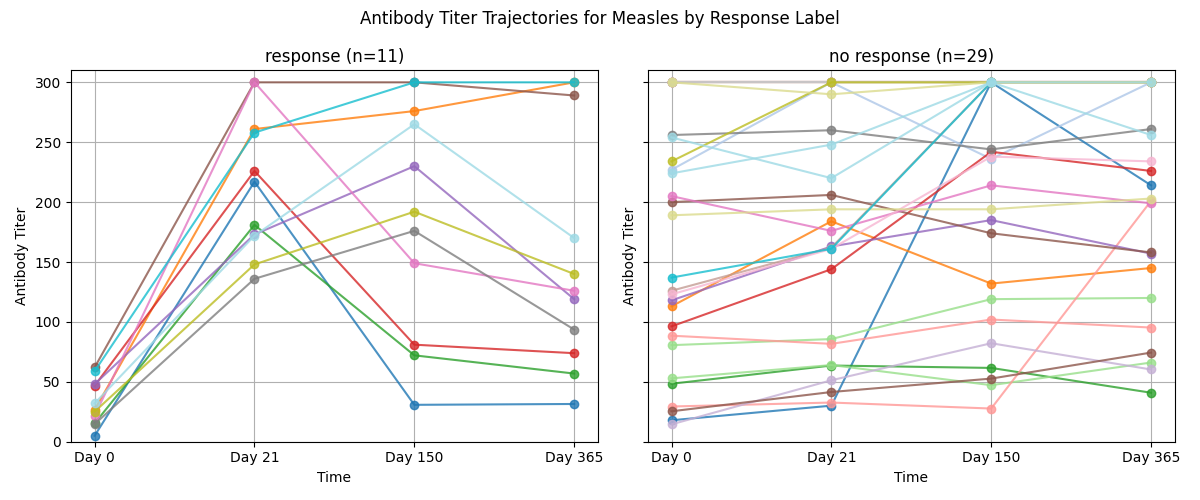
\includegraphics[width=1.1\textwidth]{images/Antibody_Titer_Trajectories_for_Measles_by_Response_Label.png}
\caption[Antibody Titer Trajectories by Response Label]{Antibody titer trajectories for each subject, colored by final response label. Subjects labeled as \texttt{response} are shown in the plot on the left, while those labeled as \texttt{no response} are shown on the right.  The initial trajectory can be traced by following the color.}
\label{fig:titer_response_label}
\end{figure}

\begin{figure}[H]
\centering
\hspace*{-1cm}
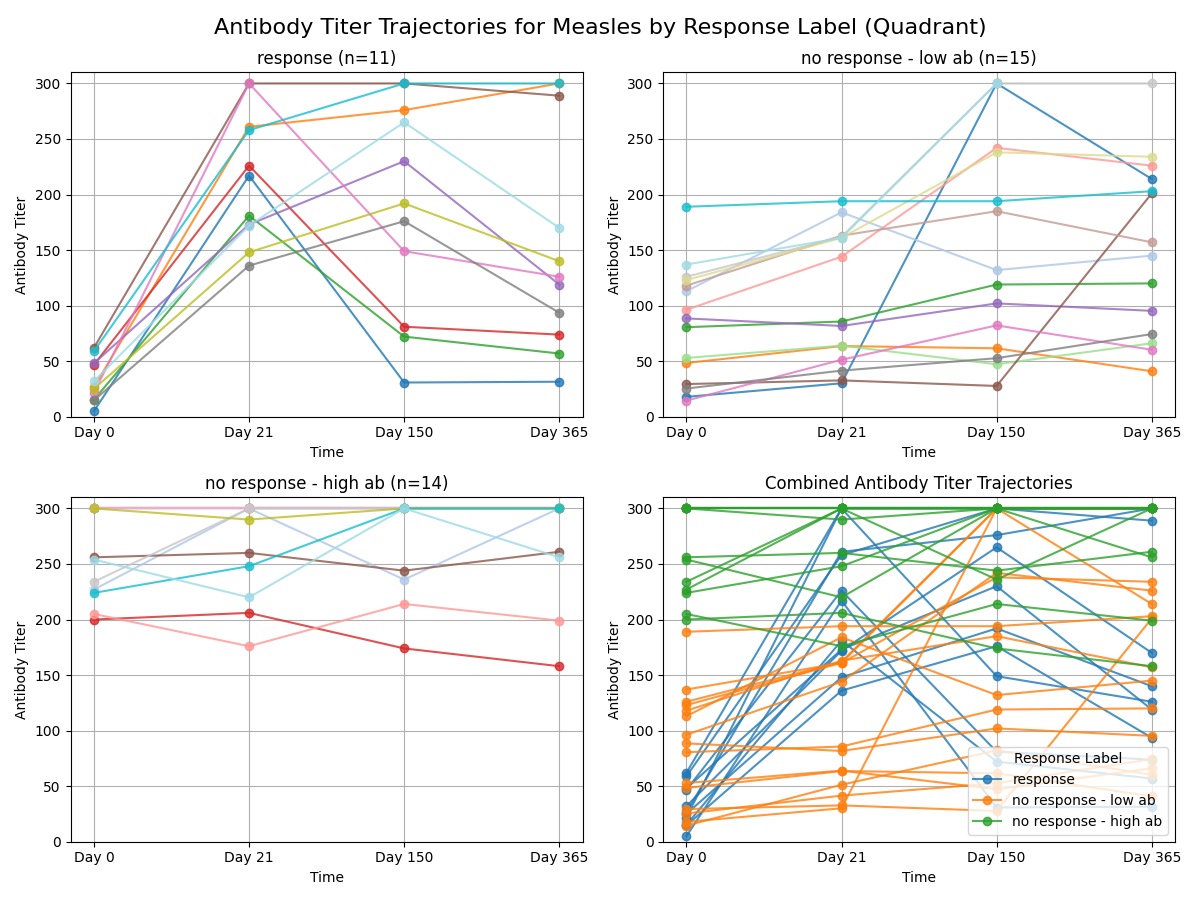
\includegraphics[width=1.1\textwidth]{images/Antibody_Titer_Trajectories_for_Measles_by_Original_Label_(Quadrant).png}
\caption[Antibody Titer Trajectories by Original Label (Quadrant)]{Antibody titer trajectories for each subject, colored by the original qualitative labels (quadrant). The plots show a clear differences in antibody responses, with responders displaying a sharp initial increase followed by gradual decline, while non-responders maintain consistently low or high titers.}
\label{fig:titer_original_label}
\end{figure}

\noindent
The simplified \texttt{response\_label} variable is used throughout the thesis as the target for classification tasks. This choice reduces the interpretability concerns. While the dataset initially contained more nuanced labels (e.g., distinguishing \texttt{no response - high ab} from \texttt{no response - low ab}), combining them into a single \texttt{no response} category improves the feasibility of training robust machine learning models given the limited sample size.

\pagebreak

\section{Correlation Analysis Within Individual Datasets}
\label{sec:correlation_analysis_within_individual_datasets}
\noindent
In an exploratory phase to gain familiarity with the data, I played around with Principal Component Analysis (PCA) to the full feature set, particularly focusing on the cytokines dataset. Although this analysis was not a definitive or robust evaluation, it provided valuable insights by showing that the first 10 principal components captured the majority of the variance. This finding suggests that much of the dataset’s information can be summarized in fewer dimensions and indicates a high degree of redundancy among features. This observation led me to believe that similar correlations likely exist in the other datasets as well. Additionally, when I performed cross-validation using a Random Forest classifier on both the full and reduced feature sets, I observed that the balanced accuracy scores hovered near 50\%. The model tended to predict only the majority class, even though the overall accuracy appeared acceptable due to class predominance. These preliminary findings underscore the challenges of high dimensionality, multicollinearity, and class imbalance that need to be addressed in subsequent predictive modeling efforts.\\
\\
Following this, I delved deeper into understanding how the variables interrelate across the different data sources. As said earlier the study comprises five distinct datasets capturing various aspects of the immune response: cytokines, cytometry, clonal breadth (TCR metrics), clonal depth (TCR metrics), and RNA data. Since each dataset represents a unique facet of immunity, I first investigated correlations within each individual dataset. Next, I concatenated the datasets to perform an integrated correlation analysis. This strategy allowed me to uncover both within-modality and cross-modality relationships, facilitating effective clustering of the data and providing the models with informative, explanatory features.
\subsection{Methodology}

\todo{Check if correct...}
\noindent
In my analysis, I use a Weighted Gene Co-expression Network Analysis (WGCNA) framework to identify modules of highly correlated features. First, I compute a correlation matrix from the data, which quantifies the pairwise relationships between features. This correlation matrix is then transformed into a distance matrix by taking one minus the absolute correlation value, ensuring that strongly correlated features are considered close. Instead of relying on a fixed linkage method like Ward.D2, WGCNA integrates hierarchical clustering with network analysis to detect modules, or clusters, of co-expressed features. In the implementation, I use the \texttt{flashClust} package for efficient hierarchical clustering, and then apply a dynamic tree cut procedure to define the modules. The modules are further visualized by assigning each a unique color using WGCNA’s labeling functions and displaying the resulting dendrogram and heatmap plots. This approach captures complex correlation patterns, effectively groups similar features.

\pagebreak
\subsection{Cytokine Data}
\begin{figure}[H]
  \centering
  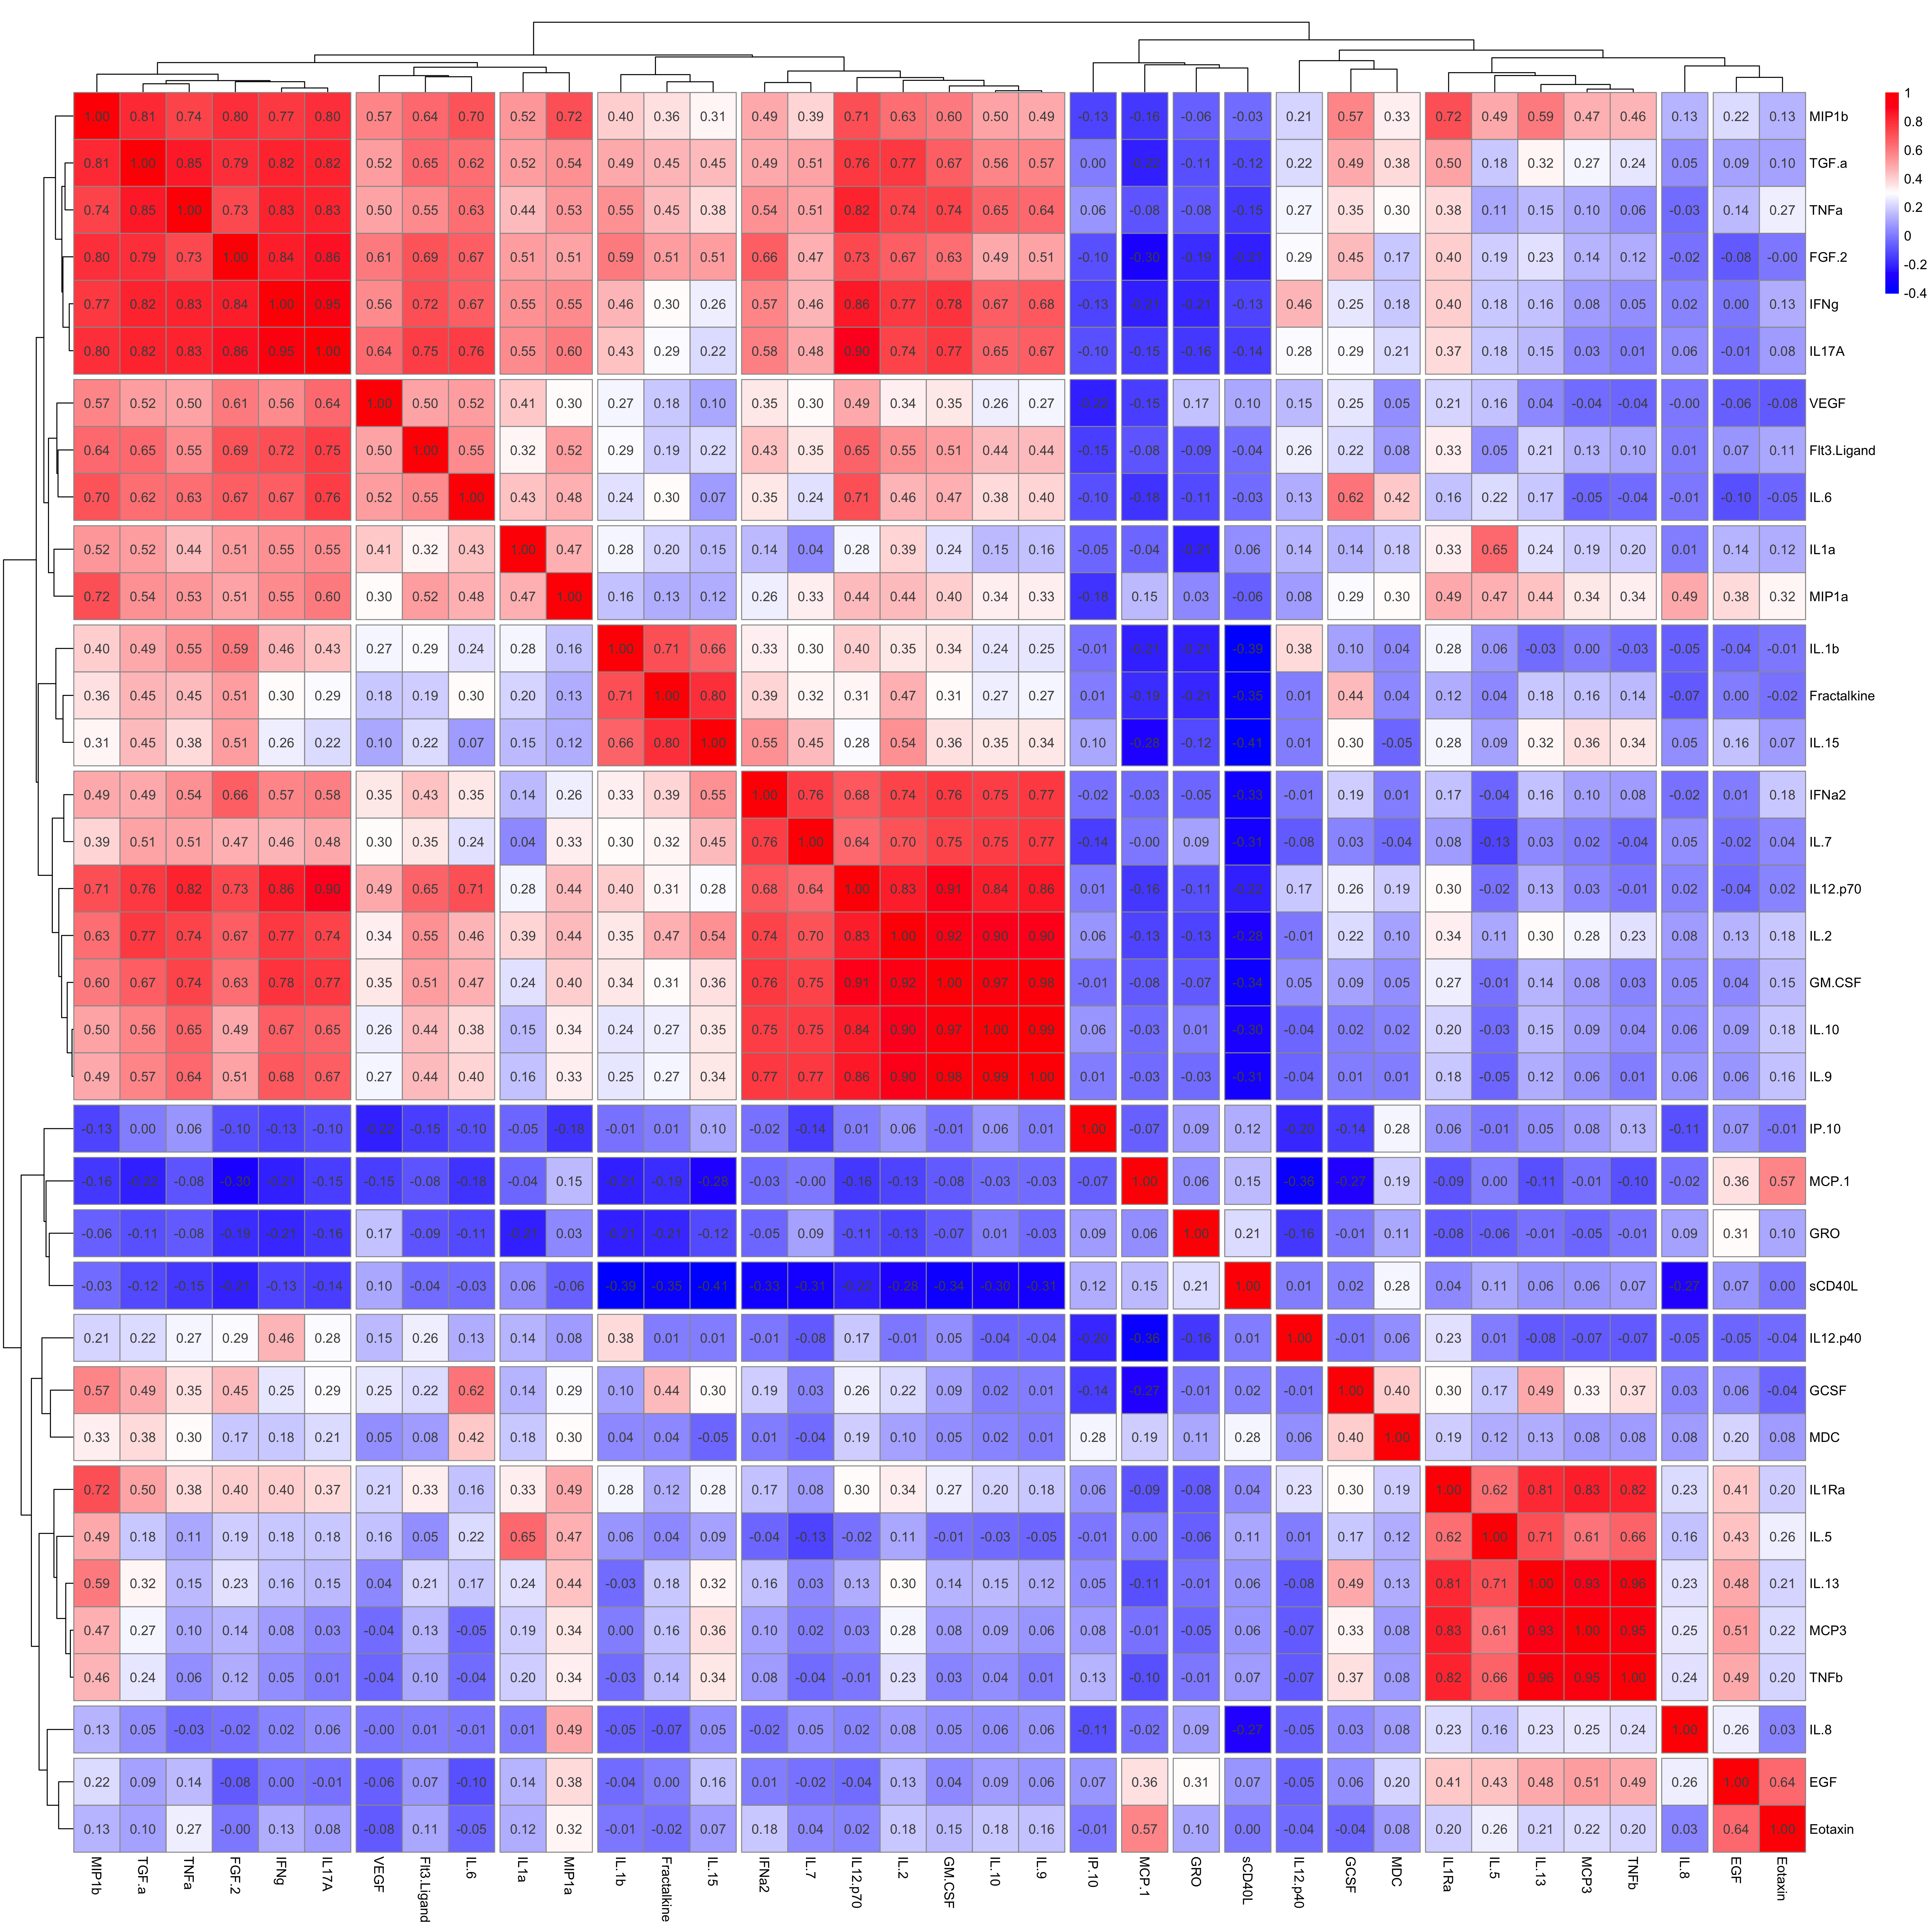
\includegraphics[width=0.8\textwidth]{images/Cytokine_euclidean_distance.png}
  \caption[cytokines data correlations]{Correlation heatmap of the cytokine data using  WGCNA hierarchical clustering.}
  \label{fig:cytokine_heatmap}
\end{figure}

The following cytokine clusters were obtained from the WGCNA hierarchical clustering analysis. The clustering reveals groups of cytokines with high inter-correlation, suggesting potential co-regulation or shared functional pathways.

\begin{table}[h!]
    \centering
    \begin{tabular}{ll}
        \textbf{Cluster 1:} & MIP1$\beta$, TGF-$\alpha$, TNF-$\alpha$, FGF-2, IFN-$\gamma$, IL17A. \\
        \textbf{Cluster 2:} & VEGF, Flt3 Ligand, IL-6. \\
        \textbf{Cluster 3:} & IL1$\alpha$, MIP1$\alpha$. \\
        \textbf{Cluster 4:} & IL-1$\beta$, Fractalkine, IL-15. \\
        \textbf{Cluster 5:} & IFN$\alpha$2, IL-7, IL12-p70, IL-2, GM-CSF, IL-10, IL-9. \\
        \textbf{Cluster 6:} & IL1Ra, IL-5, IL-13, MCP3, TNF$\beta$. \\
        \textbf{Cluster 7:} & GCSF, MDC. \\
        \textbf{Cluster 8:} & EGF, Eotaxin.
    \end{tabular}
    \caption{Cytokine Clusters}
    \label{tab:cytokine_clusters}
\end{table}


\subsection{Cytometry Data}

\begin{figure}[H]
  \centering
  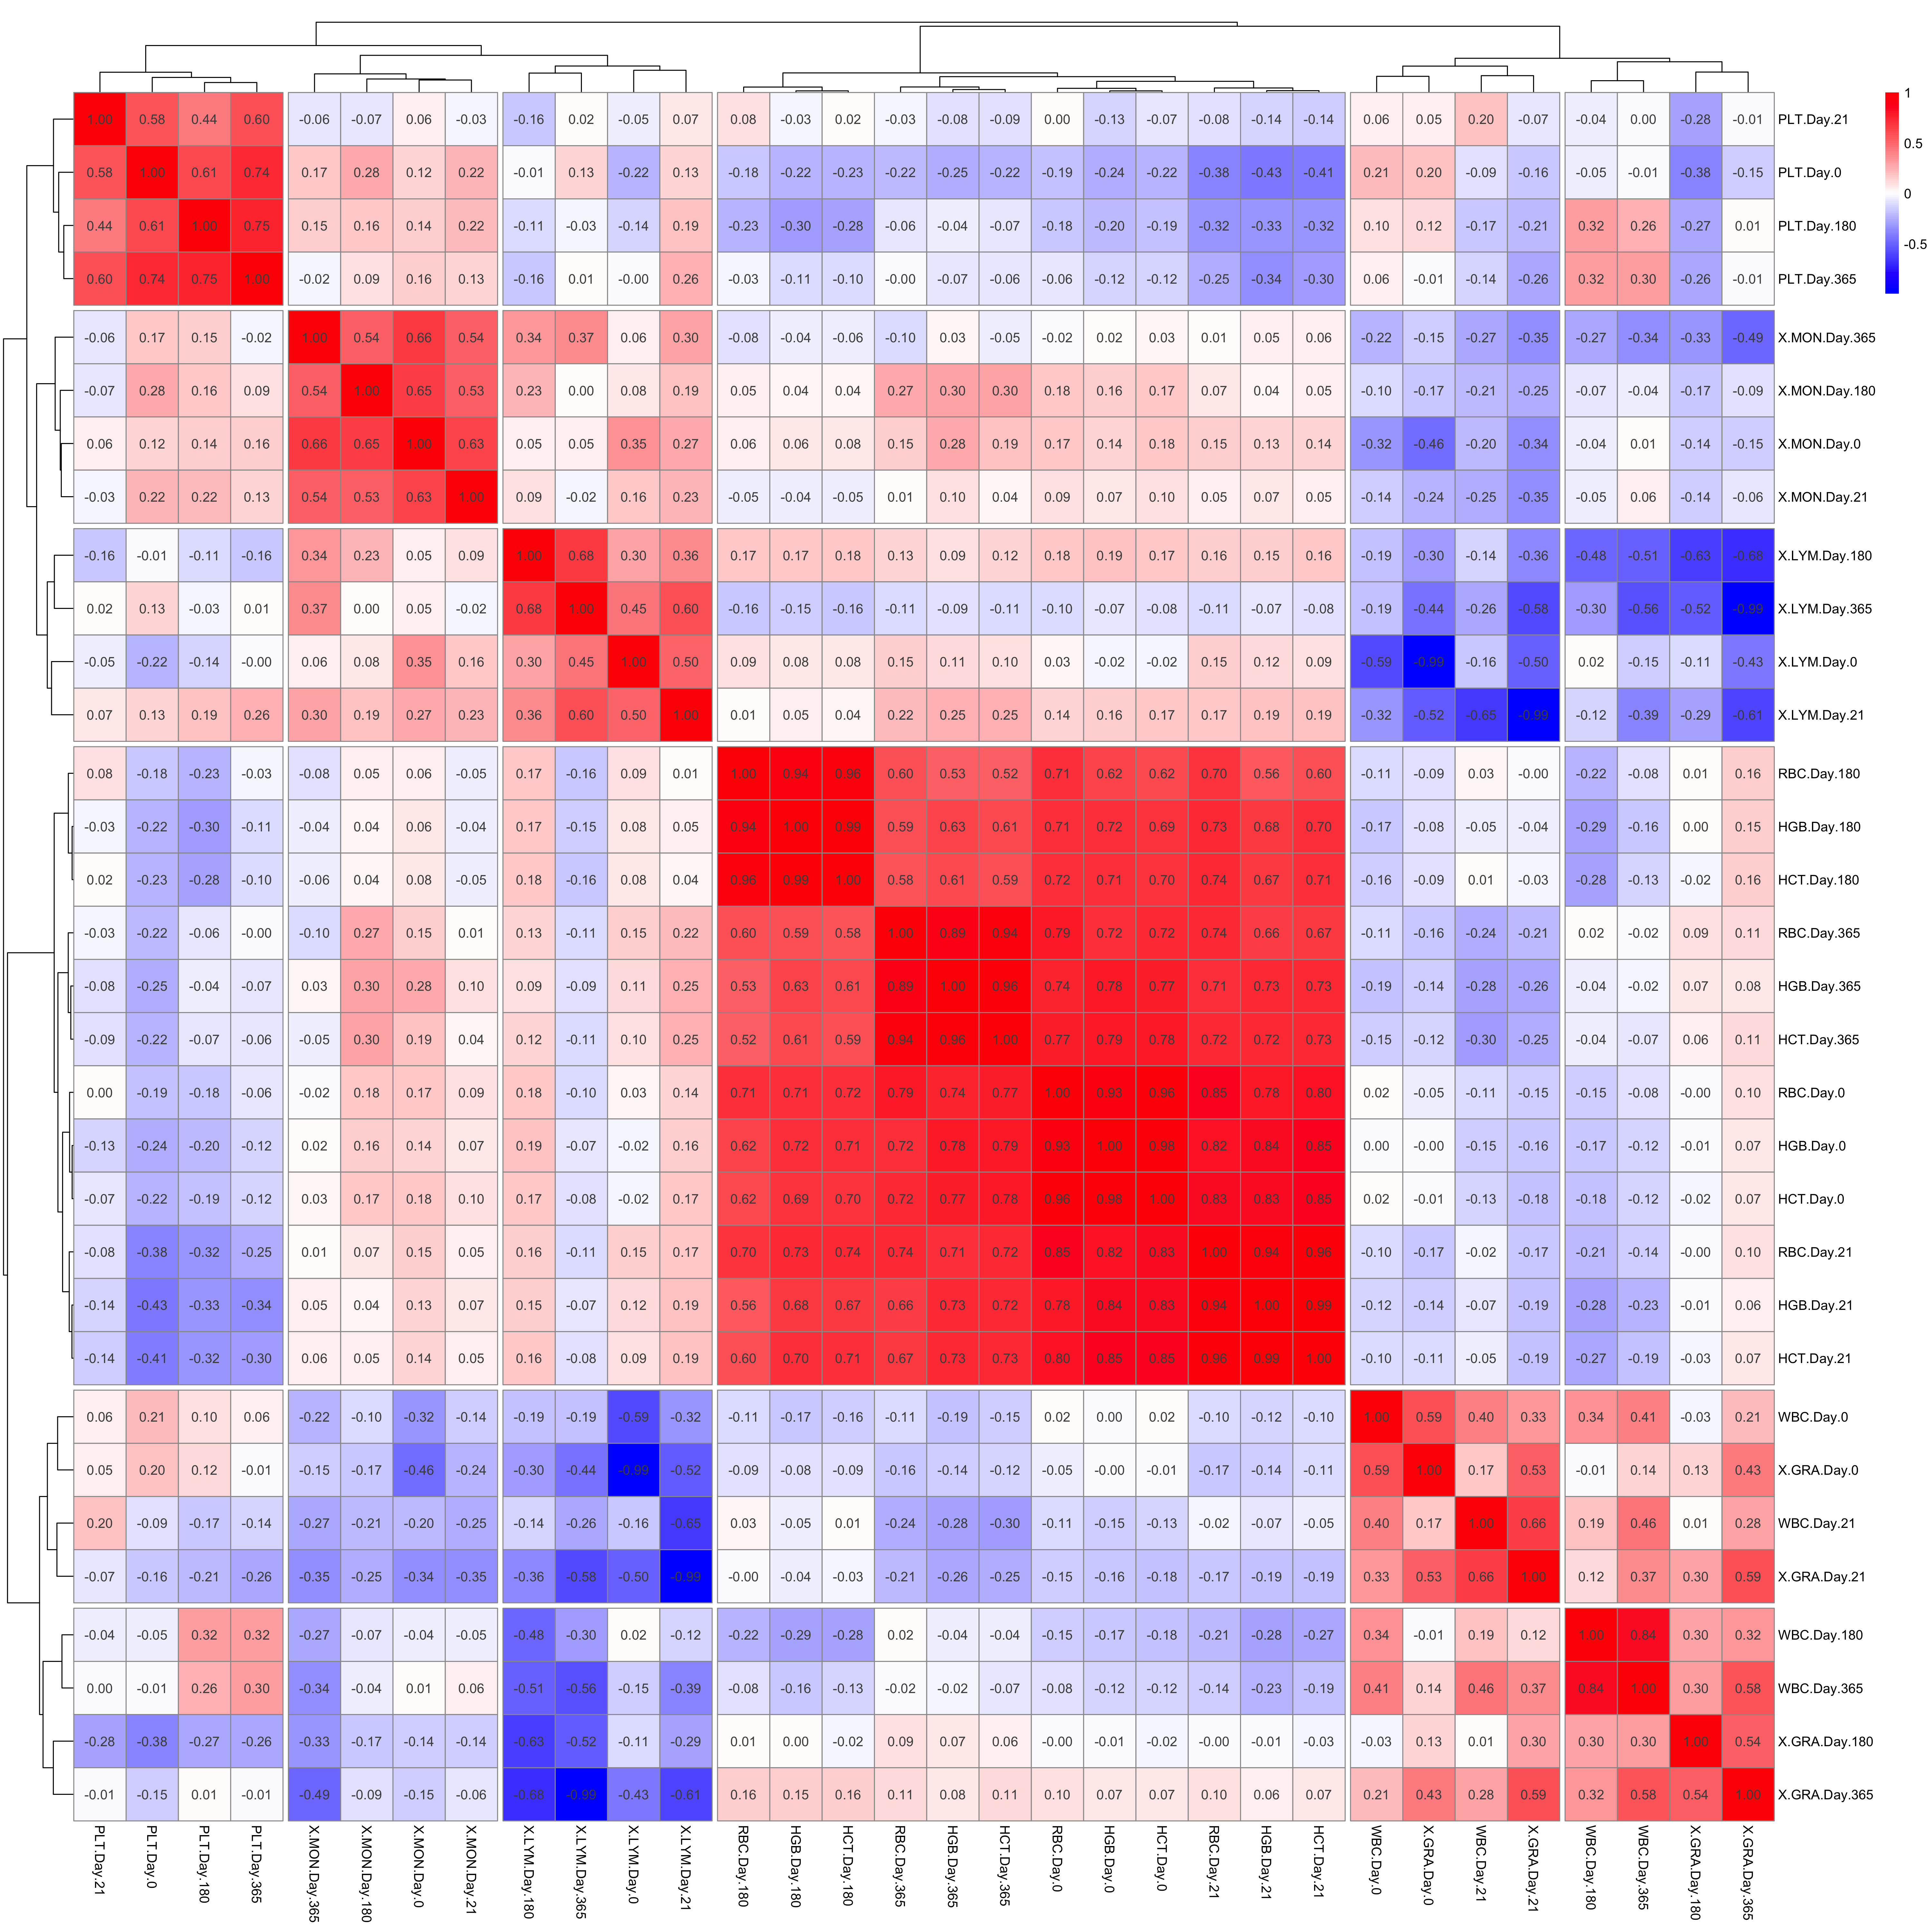
\includegraphics[width=0.8\textwidth]{images/Cytometry_euclidean_distance.png}
  \caption[cytometry data correlations]{Correlation heatmap of the cytometry data using  WGCNA hierarchical clustering.}
  \label{fig:cytometry_heatmap}
\end{figure}
\subsection{TCR Metrics}
\noindent
At Day~1, the heatmap reveals high correlation coefficients (e.g., 0.89--0.99) among RBC, HGB, and HCT, and similar correlation patterns emerge at Day~0, Day~21, Day~180, and Day~365, reinforcing their consistent co-variation over time. Even when only Day~1 is considered.
\begin{table}[h!]
    \centering
    \begin{tabular}{ll}
        \textbf{Cluster 1:} &  RBC, HGB, HCT
    \end{tabular}
    \caption{Cytokine Clusters}
    \label{tab:cytokine_clusters}
\end{table}



\subsection{RNA Data}
\begin{figure}[H]
  \centering
  \includegraphics[width=0.8\textwidth]{images/circos_RNA_only.png}
 \caption[RNA data correlations circular]{Circular correlation plot of the RNA data using. Each feature is represented along the outer edge, with colored lines indicating correlations between features (blue for positive correlations, red for negative correlations). The dense network of lines highlights the complexity of the dataset and the difficulty in visually identifying specific patterns or clusters.}
  \label{fig:RNA_circos}
\end{figure}


The RNA dataset presented a greater challenge for correlation analysis due to the high dimensionality, with a total of 382 features. To explore potential relationships within this data, I employed various visualization techniques, including the circular plot shown above.\\
\\
 Although the plot provides a comprehensive overview of all possible correlations, the dense web of lines makes it difficult to discern specific patterns or clusters visually. However, the primary advantage of this visualization is that it allows for the identification of broad trends and the detection of features that may be particularly well-connected or influential.

\begin{figure}[H]
  \centering
  \includegraphics[width=0.8\textwidth]{images/RNA_euclidean_distance.png}
  \caption[RNA data correlations]{Correlation heatmap of the RNA data using  WGCNA hierarchical clustering.}
  \label{fig:RNA_heatmap}
\end{figure}

\noindent
The same heatmap visualization technique as used before was applied to the RNA dataset, using a total of 36 cuts to correspond to the 36 different RNA modules identified through WGCNA hierarchical clustering. Selecting 36 cuts was challenging, but this number provided a reasonable balance between capturing distinct clusters and maintaining interpretability. The heatmap displays clear blocks of correlated features, with red indicating positive correlations and blue indicating negative correlations. 
\todo{@Fabio - Do I include a huge table of the clusters, because that does not seem that usefull.}

\remark{I think you can put it in the supplemental}

%%%%%%%%%%%%%%%%%%%%%%%%%%%%%%%%%%%%%%%%%%%%%%%%%%%%%%%%%%%%%%%%%%%%%%%%%%%%%%%%%%%%%%%%%%%%%%%%%%%%%%%%%%%%%%%%%%%%%%%%%%%%%%%%%%%%%%%%%%%%%%%%%





\chapter{Methodology: Modeling and Feature Selection for Measles}
%%%%%%%%%%%%%%%%%%%%%%%%%%%%%%%%%%%%%%%%%%%%%%%%%%%%%%%%%%%%%%%%%%%%%%%%%%%%%%%%%%%%%%%%%%%%%%%%%%%%%%%%%%%%%%%%%%%%%%%%%%%%%%%%%%%%%%%%%%%%%%%%%
%\todo{Explain your pipeline for exploratory analysis, model building, and selection of stable predictive features, highlighting the specific challenges and how they were overcome.}
\section{Consensus Model Approach}
\noindent
In the initial phase of the modeling process, I opted for a consensus model approach to leverage the complementary strengths of multiple predictive models. This technique involves training several distinct models independently on the different datasets and then concatenating their responses to form a unified prediction. The reason behind this approach is that different models may capture unique aspects of the data or be sensitive to different feature sets, thus enhancing the overall robustness and generalizability of the predictions.\\
\\
\todo{today-: differ from conventional consensus model}
By combining model outputs, the consensus approach aims to mitigate individual model biases and reduce the risk of overfitting, particularly given the high-dimensional nature and small size of the dataset. This method also allows for the identification of stable predictive features across models, providing insights into which features consistently contribute to predictive performance. However, the complexity introduced by this approach requires careful consideration of how model outputs are integrated and evaluated. 

\begin{figure}[H]
  \centering
  \hspace*{-0.9cm}
  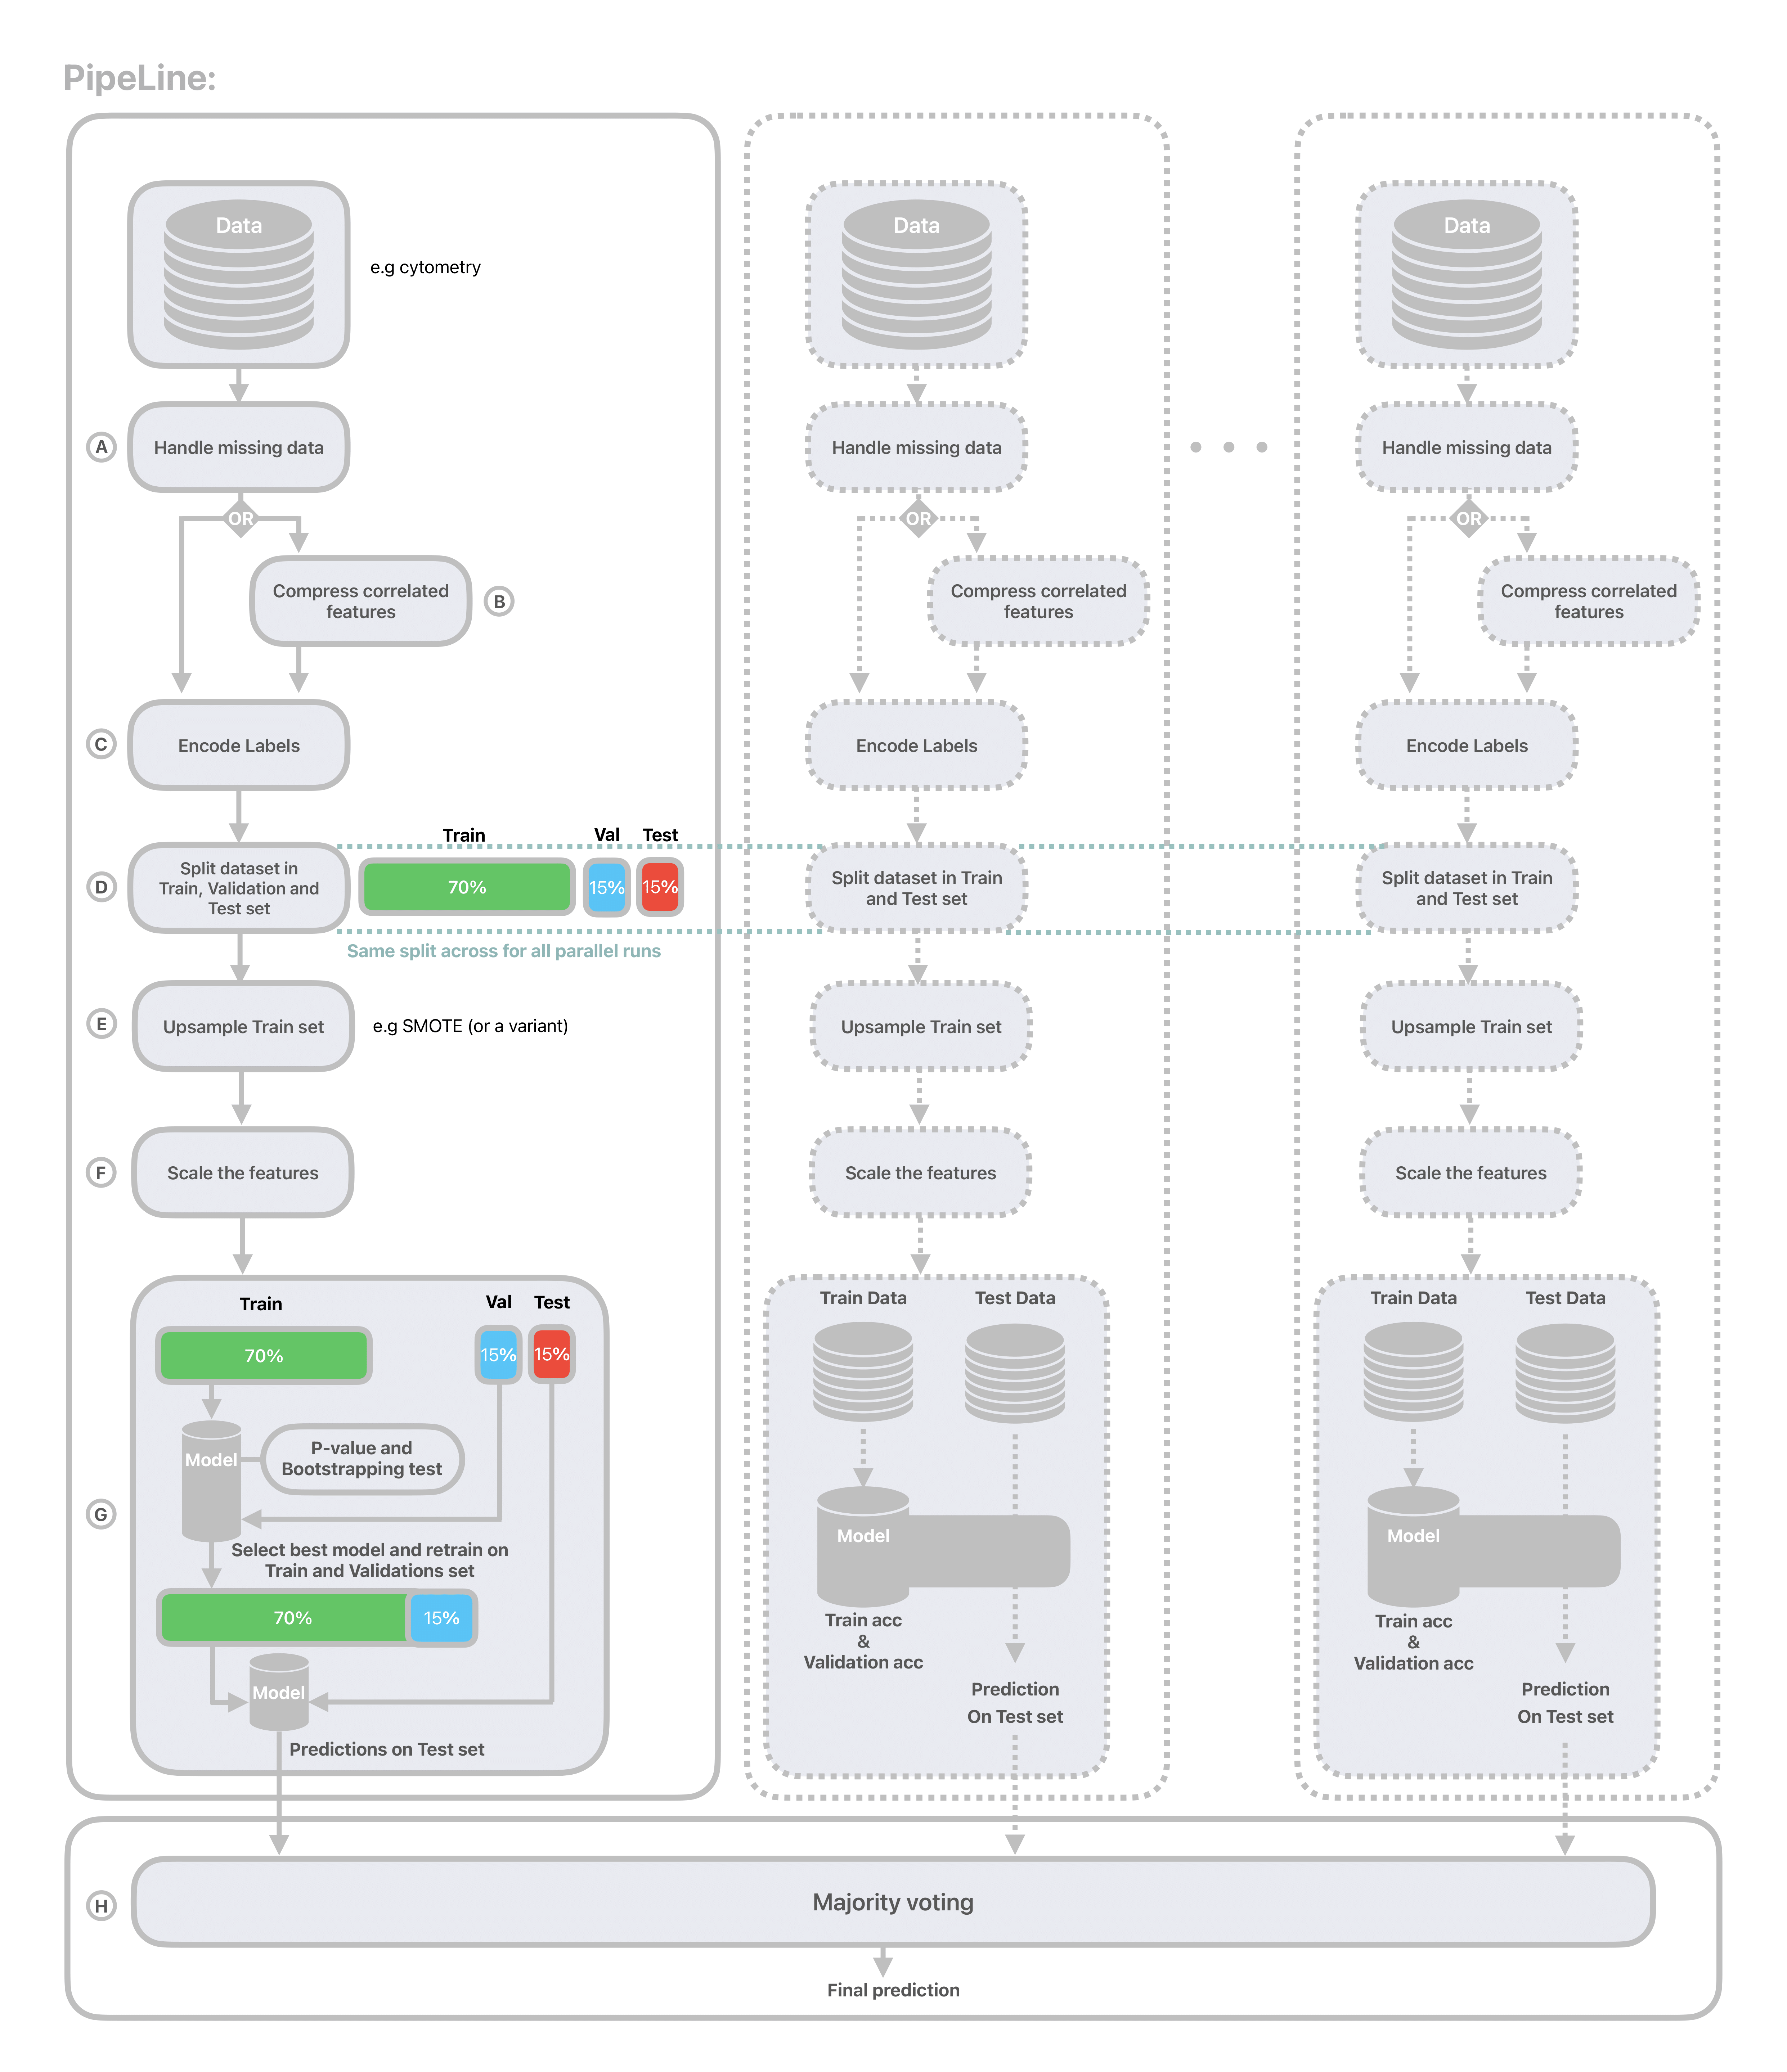
\includegraphics[width=1.1\textwidth]{images/Pipeline-1.png}
  \caption[Consensus model pipeline diagram]{The diagram illustrates the multi-model pipeline used for prediction. Each individual model follows a standardized preprocessing workflow: handling missing data, compressing correlated features, encoding labels, splitting the dataset, upsampling the training set (e.g., using SMOTE or a variant), and scaling features. The trained models then produce predictions, which are evaluated based on training and testing accuracy. Additionally, validation is performed using p-value assessment and bootstrapping to ensure robustness. The final prediction is obtained through majority voting, aggregating predictions from all models to produce a consensus output.}
  \label{fig:pipeline-1}
\end{figure}

\subsection{Pipeline Structure for Heterogeneous Datasets}
\noindent
This section details the structure applied within the consensus modeling framework. Specifically, five parallel pipelines were executed, each dedicated to one of the following distinct data types:
Cytokine measurements, Cytometry data, T-cell clonal breadth metrics, T-cell clonal depth metrics and RNA sequencing data.\\
\\
Although each pipeline starts with different data to capture unique biological insights, maintaining consistency across them is essential. Therefore, the same standardized workflow is applied to all five pipelines after loading their specific data. Using this uniform process ensures each distinct data type is handled the same before the final predictions are combined. As illustrated in Figure~\ref{fig:pipeline-1}, the standardized workflow applied to each dataset involves the following sequential steps:

\subsubsection*{Handle missing data \hyperref[fig:pipeline-1]{(A)}}
There was incomplete data in the T-cell clonal breadth and depth datasets. Unlike the cytokine, cytometry, and RNA datasets, which included records for the full cohort of 40 patients, these two datasets were missing records for entire patients. To enable consistent downstream analysis across all five pipelines using the same set of 40 samples, a procedure was employed to impute the complete feature vectors for these missing patient records.\\
\\
The core strategy leveraged the known response labels (e.g., responder/non-responder) for the complete patient cohort. First, patients absent from the clonal breadth or depth dataset but present in the full 40-sample cohort were identified. These missing patients were then conceptually grouped by their known response label. The rationale was that imputation for a missing patient should ideally reflect patterns observed in existing patients with the same outcome (e.g., imputing a missing 'responder' based on existing 'responders'). To perform the imputation, a SimpleImputer model using the mean imputation strategy was employed. This model was trained on the feature data from the available patients within the dataset and subsequently used to generate the feature values for the missing patients within their respective response groups.\\
\\
While this imputation method ensures a consistent sample size, several potential limitations must be acknowledged. Primarily, generating entire patient records introduces synthetic data that may not fully capture true biological variability or complex feature interdependencies. Furthermore, guiding the imputation by response label relies on the assumption that feature profiles differ sufficiently between response groups; if this assumption is weak, the approach could introduce bias. The reliability of the imputed values also depends fundamentally on the quality and representativeness of the existing data used to train the imputer. Consequently, incorporating these imputed samples into downstream analyses carries the risk of influencing results, potentially by altering feature distributions, reducing variance (a known effect of mean imputation), or even overestimating model performance if the imputation unintentionally increases correlations with the response variable. Therefore, the findings from these 2 models are interpreted with these limitations in mind.

\subsubsection*{Compress correlated features \hyperref[fig:pipeline-1]{(B)}}
This pipeline step focuses on addressing highly correlated features within each dataset, based on the findings presented in Section~\ref{sec:correlation_analysis_within_individual_datasets}. To mitigate potential multicollinearity issues, these identified features were subsequently compressed into a single dimension using Principal Component Analysis (PCA), resulting in one principal component that represented them in the 'compressed' feature set.\\
\\
To investigate whether feature compression impacted the final consensus model's performance, the modeling pipeline following this step was executed using two parallel approaches for each dataset. One approach utilized the original, full set of features, while the other used the reduced feature set. While addressing correlated features can potentially reduce redundancy and improve model stability, the main purpose of this parallel analysis was to empirically determine if this compression step offered a measurable advantage to the predictive accuracy of the overall consensus model for each specific data type.

\subsubsection*{Encode labels \hyperref[fig:pipeline-1]{(C)}}
As machine learning algorithms typically require numerical inputs, the categorical target variable was converted into a numerical format in this step. This encoding simply assigned a unique integer (e.g., 0 and 1) to each response class.

\subsubsection*{Split dataset \hyperref[fig:pipeline-1]{(D)}}
To properly evaluate model performance and ensure generalization to new data, the dataset was partitioned into three independent subsets: a training set, a validation set, and a test set.\\
\\
The partitioning followed a 70\% / 15\% / 15\% ratio, allocating the data as follows:
\begin{itemize}
    \item \textbf{Training Set (70\%):} This largest subset was used solely for training the models. The algorithms learn patterns, relationships, and parameters from this data.
    \item \textbf{Validation Set (15\%):} This independent subset was crucial during the model development phase, specifically for selecting the optimal combination of model algorithm and data preprocessing choices. Since multiple distinct model types were evaluated in parallel across the pipelines, and different up-sampling techniques were considered (detailed in the next step), this validation set was used to compare their performance. The combination of model algorithm and up-sampling method yielding the best results on the validation set was selected for final evaluation. Performing the model and up-sampling selection using the validation set is critical to ensure that the test set remains completely untouched and unseen, thereby preserving its integrity for the final, unbiased assessment of generalization performance.
    \item \textbf{Test Set (15\%):} This subset was strictly held out until all model development and selection were finalized based on the training and validation sets. It was used only once at the very end to provide a final, unbiased estimate of how the chosen model configuration is expected to perform on new, unseen data.
\end{itemize}

\subsubsection*{Up-sample Train set \hyperref[fig:pipeline-1]{(E)}}
A common challenge in biological datasets is class imbalance, where one response class (in this case, responders) may be significantly less prevalent than the other within the training data. This may cause the model to favor the majority class during training. To counteract this and evaluate different mitigation approaches, three distinct strategies for handling class imbalance were applied exclusively to the 70\% training set:

\begin{enumerate}
    \item \textbf{No Resampling with Class Weighting:} In this strategy, the training data distribution was not modified. Instead, imbalance was addressed algorithmically during model training by assigning higher weights to the minority class samples. This typically adjusts the model's loss function, making errors on minority class examples more costly and forcing the model to pay more attention to them.
    \item \textbf{Random Over-Sampling (ROS):} This method directly modifies the training set by increasing the representation of the minority class. It works by randomly selecting and duplicating existing samples from the minority class until a desired level of balance (an equal number of samples per class) is achieved.
    \item \textbf{SMOTE (Synthetic Minority Over-sampling Technique):} Generating new, synthetic minority class samples through feature space interpolation, as detailed further below and illustrated in Figure~\ref{fig:SMOTE_explained}.
\end{enumerate}

\begin{figure}[htbp]
    \centering
    % Verify path is correct
    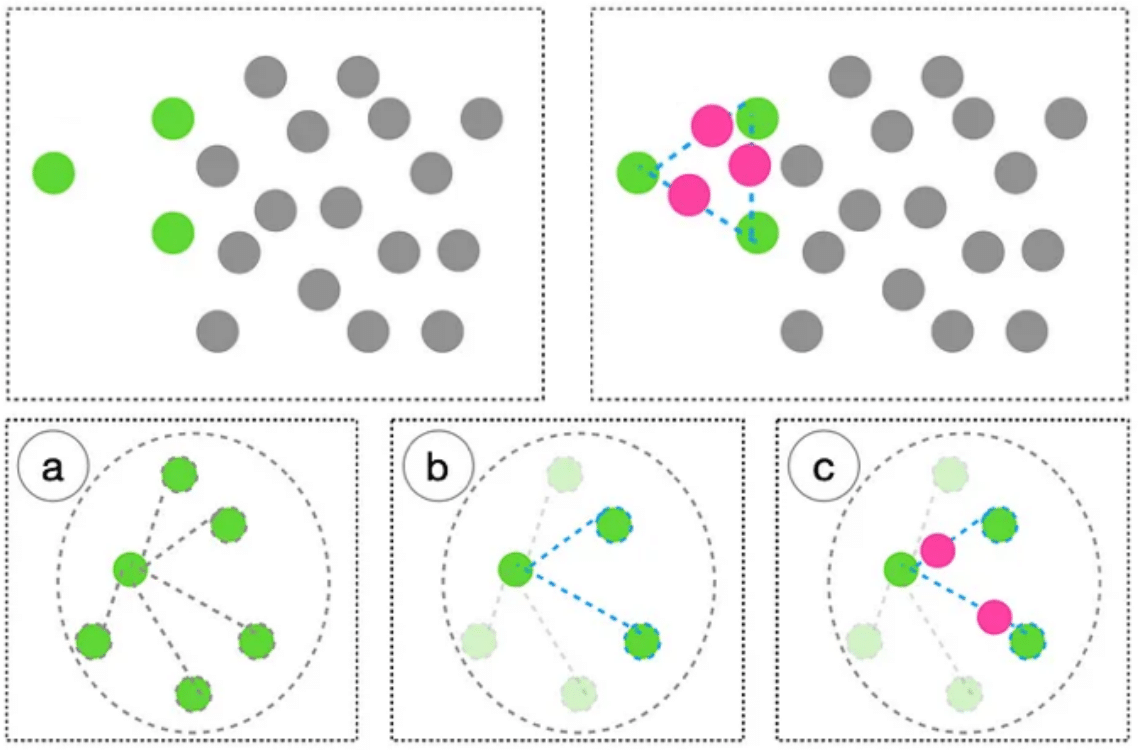
\includegraphics[width=0.8\textwidth]{images/SMOTE-explained.png}
    \caption[Illustration of the SMOTE mechanism]{Illustration of the Synthetic Minority Over-sampling Technique (SMOTE) mechanism. Top left: Initial imbalanced data distribution (minority in green, majority in gray). Top right: Generation of synthetic samples (pink) along lines connecting a minority instance to its nearest minority neighbors. Bottom row: Detailed steps showing (a) identification of k-nearest minority neighbors (here k=5), (b) selection of neighbors for synthesis, and (c) creation of synthetic samples (pink) along the vectors to selected neighbors. Figure based on figures 1 and 2 presented in \cite{Truong2022SMOTEVariants}.}
    \label{fig:SMOTE_explained} % Unique label
\end{figure}

\begin{figure}[htbp]
    \centering
    % Verify path is correct
    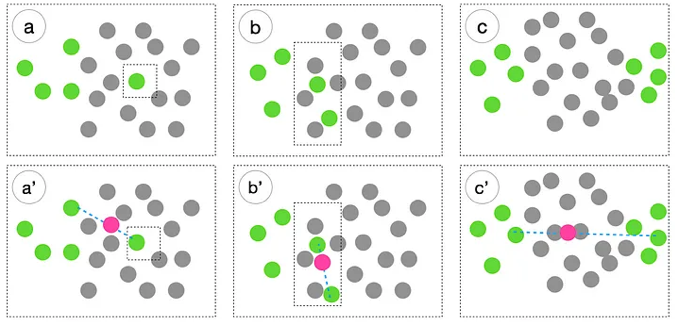
\includegraphics[width=0.8\textwidth]{images/SMOTE-weaknesses.png}
    \caption[Illustration of SMOTE weaknesses]{Conceptual illustration of potential weaknesses associated with SMOTE. The bottom row (a', b', c') depicts synthetic sample generation (pink) relative to regions shown in the top row (a, b, c). Potential issues illustrated include: (a/a') Generation influenced by potential noise or outliers (isolated minority sample). (b/b') Synthetic samples potentially overlapping with dense majority class regions due to disregard for majority sample proximity. (c/c') Generation possibly bridging distinct minority clusters, which could ignore underlying data structure or cause overgeneralization. Figure adapted from figure 4 presented in \cite{Truong2022SMOTEVariants}.}
    \label{fig:SMOTE_weaknesses} % Unique label
\end{figure}
% --- End Figures ---

% --- Detailed SMOTE Discussion (Separate Paragraphs) ---
\noindent % Start new paragraph
SMOTE \cite{Chawla2002SMOTE}, visually explained in Figure~\ref{fig:SMOTE_explained}, generates synthetic minority samples rather than simply duplicating existing ones like ROS. It selects a minority instance, finds its k-nearest minority class neighbors, and creates new samples along the line segments joining the instance to some of these neighbors. This method can potentially create a more diverse minority representation and smoother decision boundaries.\\
\\
However, SMOTE also has known limitations (illustrated conceptually in Figure~\ref{fig:SMOTE_weaknesses}), as discussed in literature \cite{Truong2022SMOTEVariants}. Potential drawbacks include overgeneralization (creating samples that blur class distinctions or ignore sub-clusters), amplification of noise if based on outlier samples, and possible generation of samples too close to or overlapping with the majority class, as the original algorithm doesn't explicitly consider majority proximity. Despite these points, SMOTE was included for comparison as a prominent synthetic data generation technique.\\
\\
The relative effectiveness of these three imbalance-handling strategies (Class Weighting, ROS, SMOTE) was assessed empirically for each model pipeline. As established during data splitting (Section~\ref{sec:datasplit} - *ensure this label is correct*), the performance metrics achieved on the 15\% validation set were used to select the optimal strategy for each model before final assessment on the test set. It is crucial to reiterate that these imbalance adjustments were applied strictly to the training data partition to maintain the integrity of the validation and test sets.









\subsubsection*{Scale the features \hyperref[fig:pipeline-1]{(F)}}
\todo{today-...}

\subsubsection*{Train the models \hyperref[fig:pipeline-1]{(G)}}
\todo{today-...}










\begin{figure}[H]
  \centering
  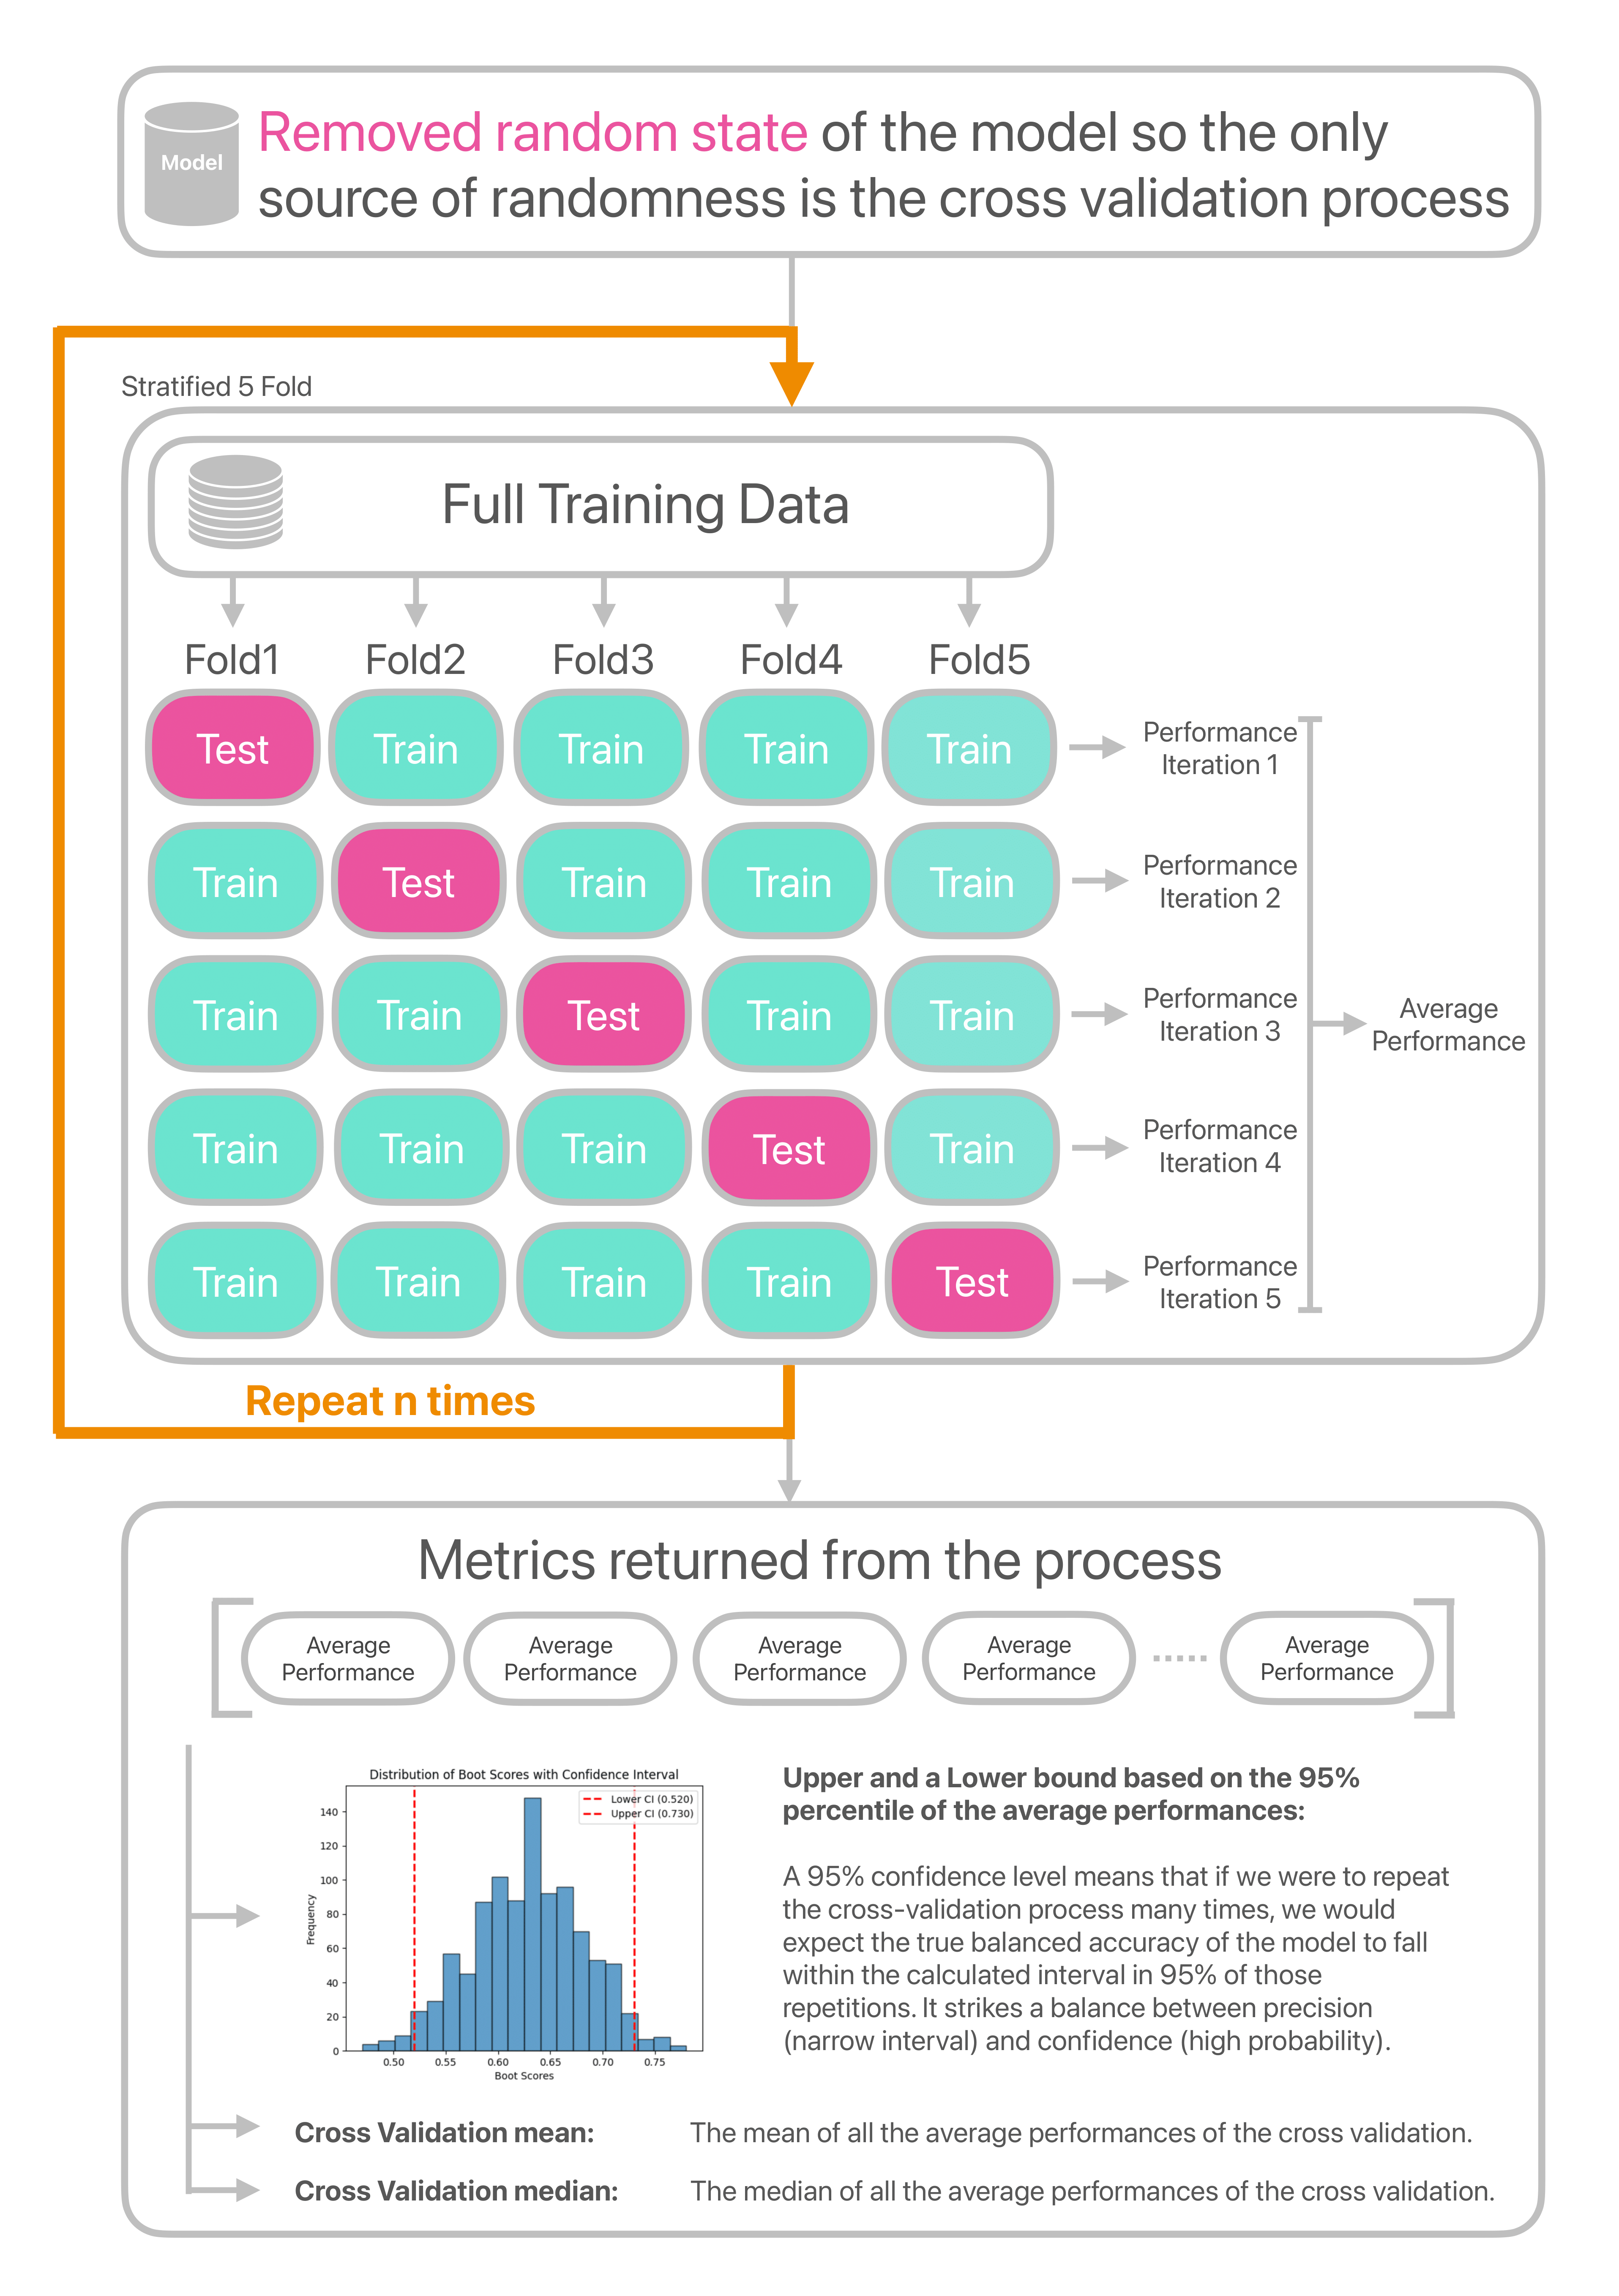
\includegraphics[width=0.9\textwidth]{images/Bootstrapping-1.png}
  \caption[Confidence interval estimation diagram using repeated stratified 5-fold cross-validation]{This diagram illustrates the process of estimating the confidence interval of a model's performance using repeated stratified k-fold cross-validation. Initially, the model's random state is removed to ensure the cross-validation process is the sole source of randomness. Stratified k-fold cross-validation (k=5) is used to evaluate model performance, with the average score across folds representing a single iteration's result. This entire cross-validation procedure is repeated 'n' times (e.g., 1000) to simulate the variability in performance across different random splits. The resulting 'n' average performance scores are then used to calculate the confidence interval. These bounds indicate the range within which we expect the model's true performance to lie with a high degree of confidence, providing a robust measure of the model's reliability.}
  \label{fig:Bootstrapping-1}
\end{figure}

\begin{figure}[H]
  \centering
  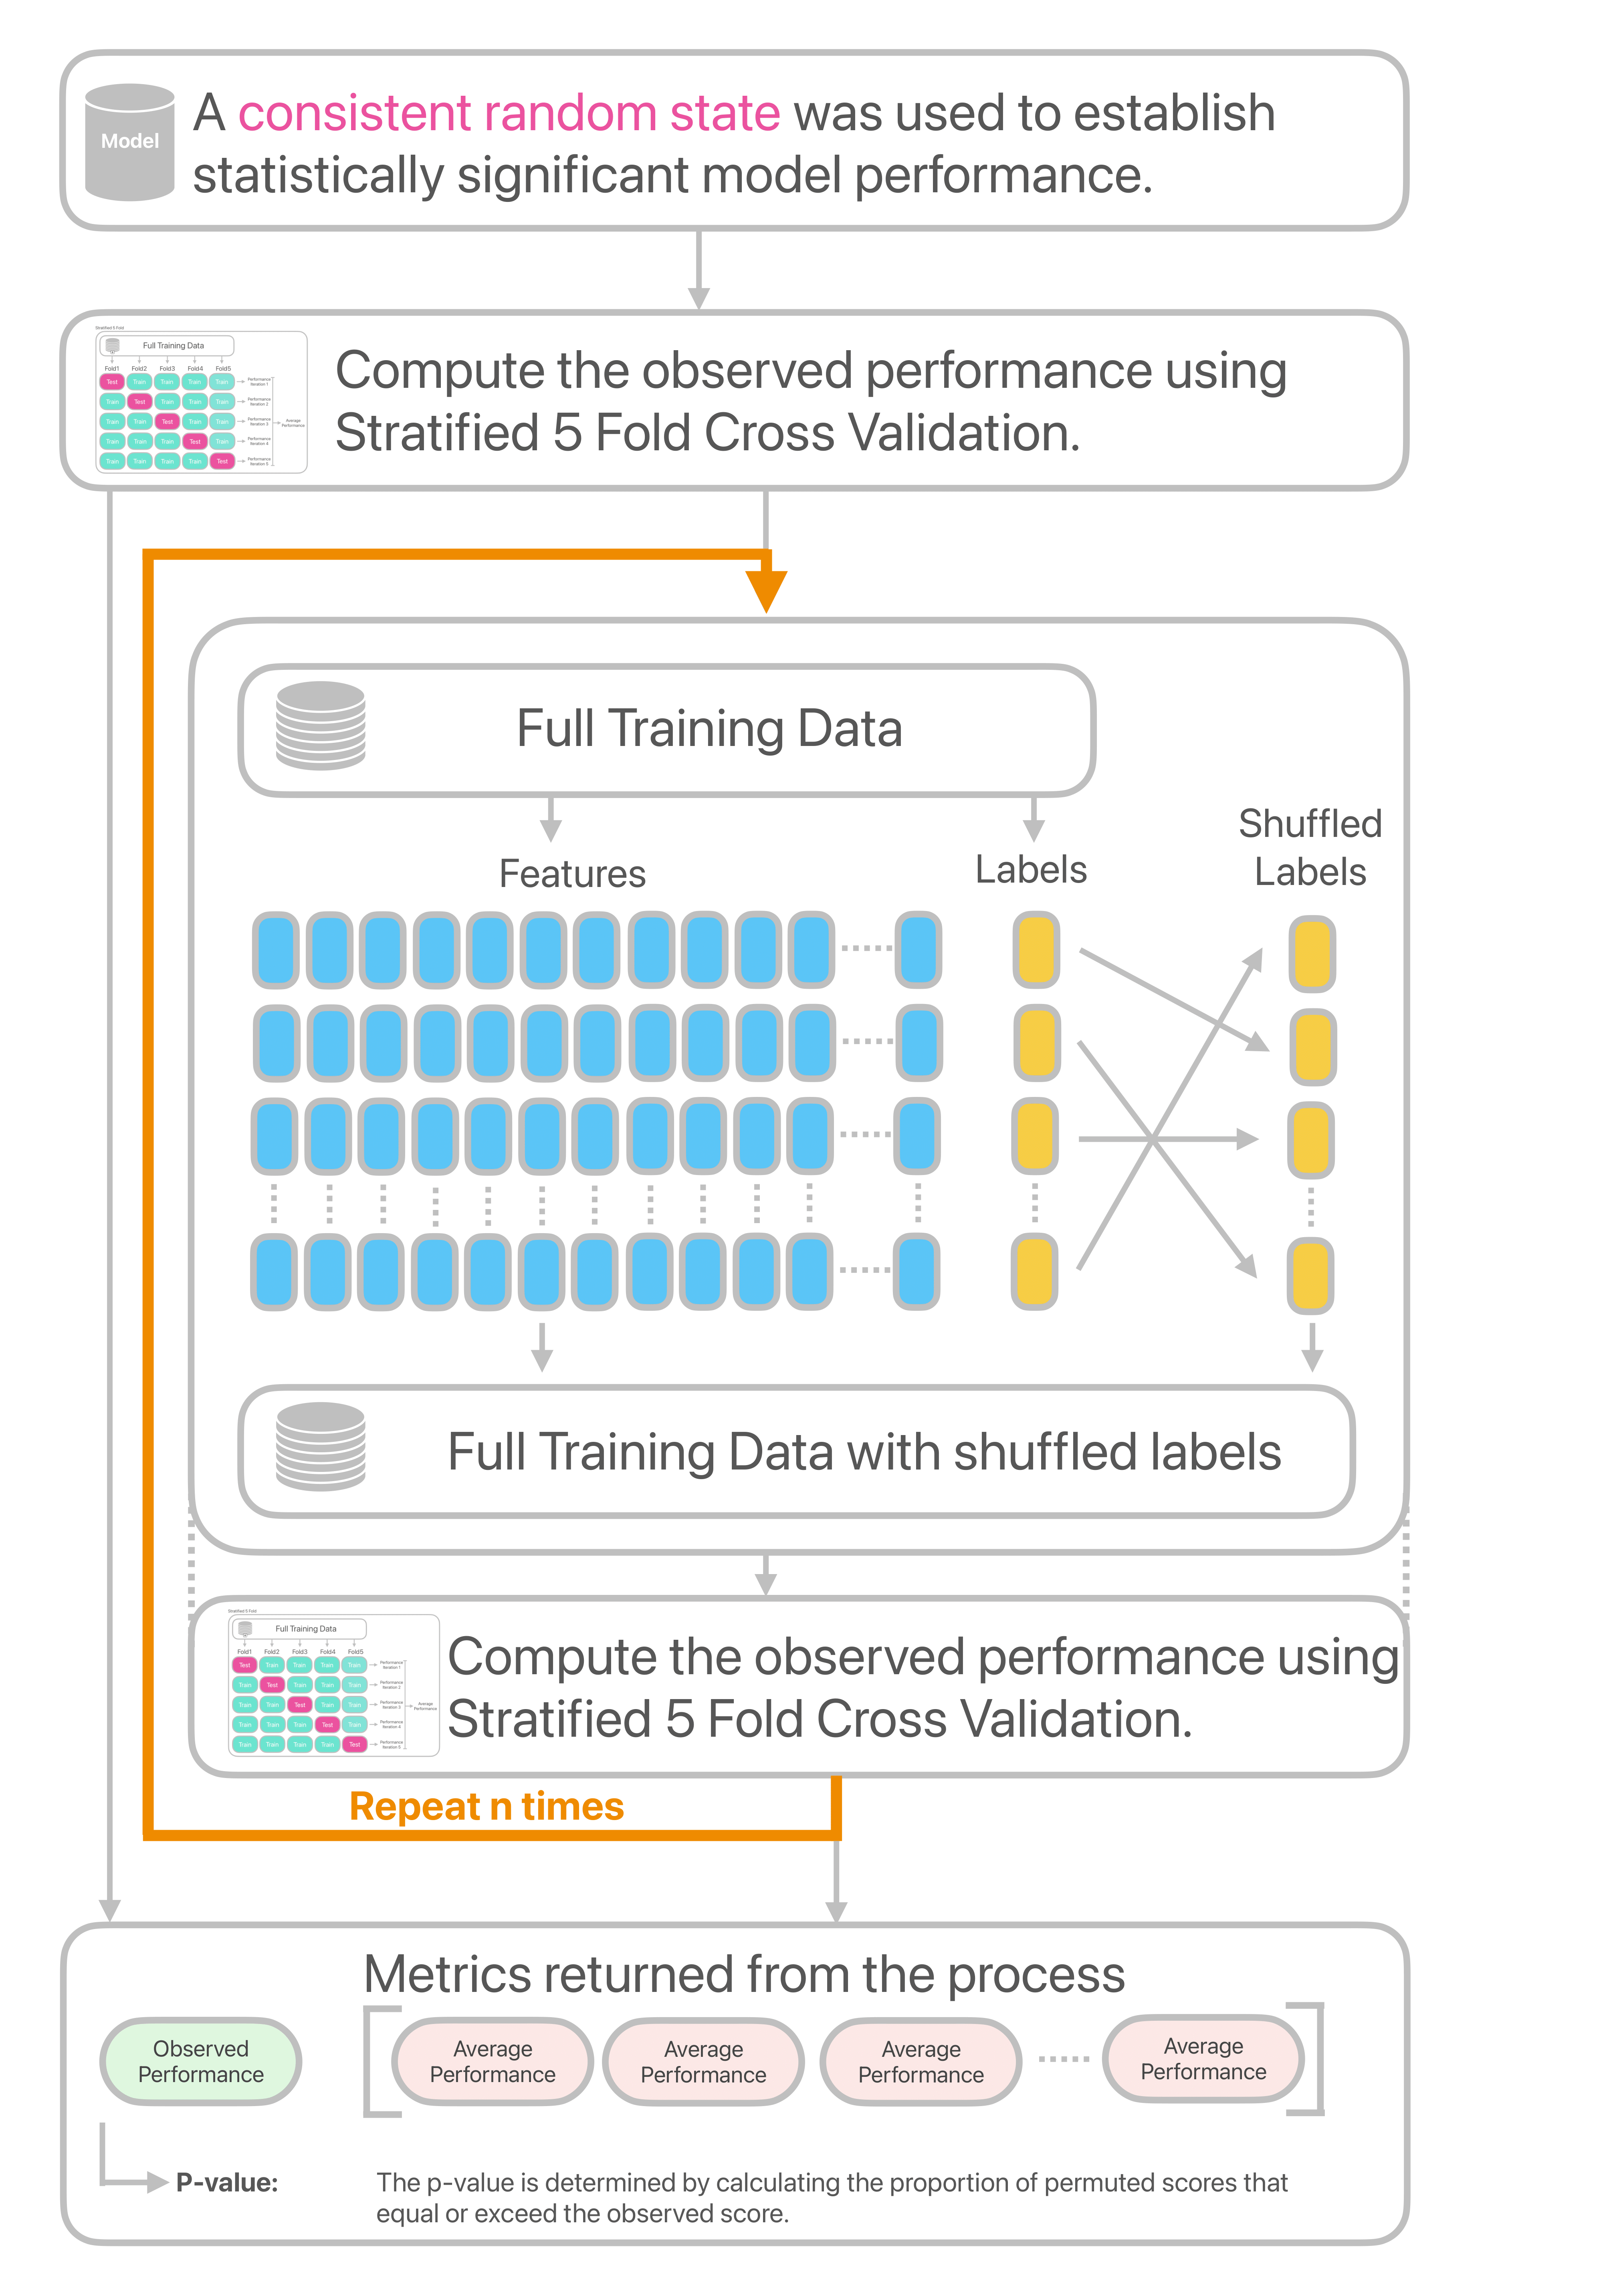
\includegraphics[width=0.9\textwidth]{images/P-value_test-1.png}
  \caption[Evaluating model significance via permutation testing and p-value calculation diagram]{This diagram illustrates a permutation test designed to evaluate the statistical significance of a model's performance. Initially, a consistent random state is set to ensure reproducible results. The model's performance is first assessed on the original data using stratified 5-fold cross-validation, yielding the 'observed performance.' Subsequently, to determine if this performance is merely due to chance, the labels are repeatedly shuffled. For each shuffled dataset, the model's performance is re-evaluated using the same stratified 5-fold cross-validation. This process is repeated 'n' times, resulting in a distribution of 'permuted performances.' Finally, the p-value is calculated as the proportion of permuted performances that equal or exceed the observed performance, indicating the likelihood of obtaining such performance by chance alone.}
  \label{fig:P-value_test-1}
\end{figure}




%%%%%%%%%%%%%%%%%%%%%%%%%%%%%%%%%%%%%%%%%%%%%%%%%%%%%%%%%%%%%%%%%%%%%%%%%%%%%%%%%%%%%%%%%%%%%%%%%%%%%%%%%%%%%%%%%%%%%%%%%%%%%%%%%%%%%%%%%%%%%%%%%





\chapter{Results for the Measles Pipeline}
%%%%%%%%%%%%%%%%%%%%%%%%%%%%%%%%%%%%%%%%%%%%%%%%%%%%%%%%%%%%%%%%%%%%%%%%%%%%%%%%%%%%%%%%%%%%%%%%%%%%%%%%%%%%%%%%%%%%%%%%%%%%%%%%%%%%%%%%%%%%%%%%%
\todo{Present model performance, feature importance, and interpretation of findings from the measles data.}
%%%%%%%%%%%%%%%%%%%%%%%%%%%%%%%%%%%%%%%%%%%%%%%%%%%%%%%%%%%%%%%%%%%%%%%%%%%%%%%%%%%%%%%%%%%%%%%%%%%%%%%%%%%%%%%%%%%%%%%%%%%%%%%%%%%%%%%%%%%%%%%%%





\chapter{Cross-Vaccine Marker Validation with Hepatitis B}
%%%%%%%%%%%%%%%%%%%%%%%%%%%%%%%%%%%%%%%%%%%%%%%%%%%%%%%%%%%%%%%%%%%%%%%%%%%%%%%%%%%%%%%%%%%%%%%%%%%%%%%%%%%%%%%%%%%%%%%%%%%%%%%%%%%%%%%%%%%%%%%%%
\todo{Describe the application of the same pipeline to the hepatitis B dataset, compare predictive features, and discuss the validation process.}
%%%%%%%%%%%%%%%%%%%%%%%%%%%%%%%%%%%%%%%%%%%%%%%%%%%%%%%%%%%%%%%%%%%%%%%%%%%%%%%%%%%%%%%%%%%%%%%%%%%%%%%%%%%%%%%%%%%%%%%%%%%%%%%%%%%%%%%%%%%%%%%%%





\chapter{Discussion and Conclusion}
%%%%%%%%%%%%%%%%%%%%%%%%%%%%%%%%%%%%%%%%%%%%%%%%%%%%%%%%%%%%%%%%%%%%%%%%%%%%%%%%%%%%%%%%%%%%%%%%%%%%%%%%%%%%%%%%%%%%%%%%%%%%%%%%%%%%%%%%%%%%%%%%%
\todo{Summarize insights, implications for vaccine response prediction, and potential future work based on the comparative analysis.}
%%%%%%%%%%%%%%%%%%%%%%%%%%%%%%%%%%%%%%%%%%%%%%%%%%%%%%%%%%%%%%%%%%%%%%%%%%%%%%%%%%%%%%%%%%%%%%%%%%%%%%%%%%%%%%%%%%%%%%%%%%%%%%%%%%%%%%%%%%%%%%%%%





\chapter{Future work}
%%%%%%%%%%%%%%%%%%%%%%%%%%%%%%%%%%%%%%%%%%%%%%%%%%%%%%%%%%%%%%%%%%%%%%%%%%%%%%%%%%%%%%%%%%%%%%%%%%%%%%%%%%%%%%%%%%%%%%%%%%%%%%%%%%%%%%%%%%%%%%%%%
%%%%%%%%%%%%%%%%%%%%%%%%%%%%%%%%%%%%%%%%%%%%%%%%%%%%%%%%%%%%%%%%%%%%%%%%%%%%%%%%%%%%%%%%%%%%%%%%%%%%%%%%%%%%%%%%%%%%%%%%%%%%%%%%%%%%%%%%%%%%%%%%%


\bibliographystyle{plain}
\bibliography{references}

\end{document}
